% !TeX encoding = UTF-8
% !TeX spellcheck = en_US
% !TeX root = presentation.tex


%%%%%%%%%%%%%%%%%%%%%%%%%%%%%%%%%%%%%%%%%%%%%%%%%%%%%%%%%%%%%%%%%%%%%%%%%%%%%%%%
{
\usebackgroundtemplate{
\includegraphics[height=\paperheight]{logos/amd-title}}
\begin{frame}[plain]
%\begin{resizepar}
%\begin{tikzpicture}
%\matrix[matrix of nodes,ampersand replacement=\&,column sep=10mm,every node/.style={anchor=center}] {
%\hspace*{1em}     \&
%\includegraphics[height=25mm]{logos/eurollvm}            \&
%
\includegraphics[height=8mm]{logos/amd-black}            \&
%\hspace*{1em}        \\
%};
%\end{tikzpicture}
%\end{resizepar}

%\vspace*{-12ex}
\titlepage
\end{frame}
}
\addtocounter{framenumber}{-1}




%%%%%%%%%%%%%%%%%%%%%%%%%%%%%%%%%%%%%%%%%%%%%%%%%%%%%%%%%%%%%%%%%%%%%%%%%%%%%%%%
\AtBeginSection[]
{
  \begin{frame}[shrink]{Outline}
    \vspace*{5ex}
    \tableofcontents[currentsection,hideothersubsections]
  \end{frame}
}


%%%%%%%%%%%%%%%%%%%%%%%%%%%%%%%%%%%%%%%%%%%%%%%%%%%%%%%%%%%%%%%%%%%%%%%%%%%%%%%%
\begin{frame}[shrink]{Outline}
\vspace*{2ex}
\tableofcontents[hideallsubsections]
\end{frame}




%%%%%%%%%%%%%%%%%%%%%%%%%%%%%%%%%%%%%%%%%%%%%%%%%%%%%%%%%%%%%%%%%%%%%%%%%%%%%%%%
%%%%%%%%%%%%%%%%%%%%%%%%%%%%%%%%%%%%%%%%%%%%%%%%%%%%%%%%%%%%%%%%%%%%%%%%%%%%%%%%
\section{Introduction}

\begin{frame}[fragile]{About Me}

\begin{columns}
\begin{column}[c]{0.38\textwidth}
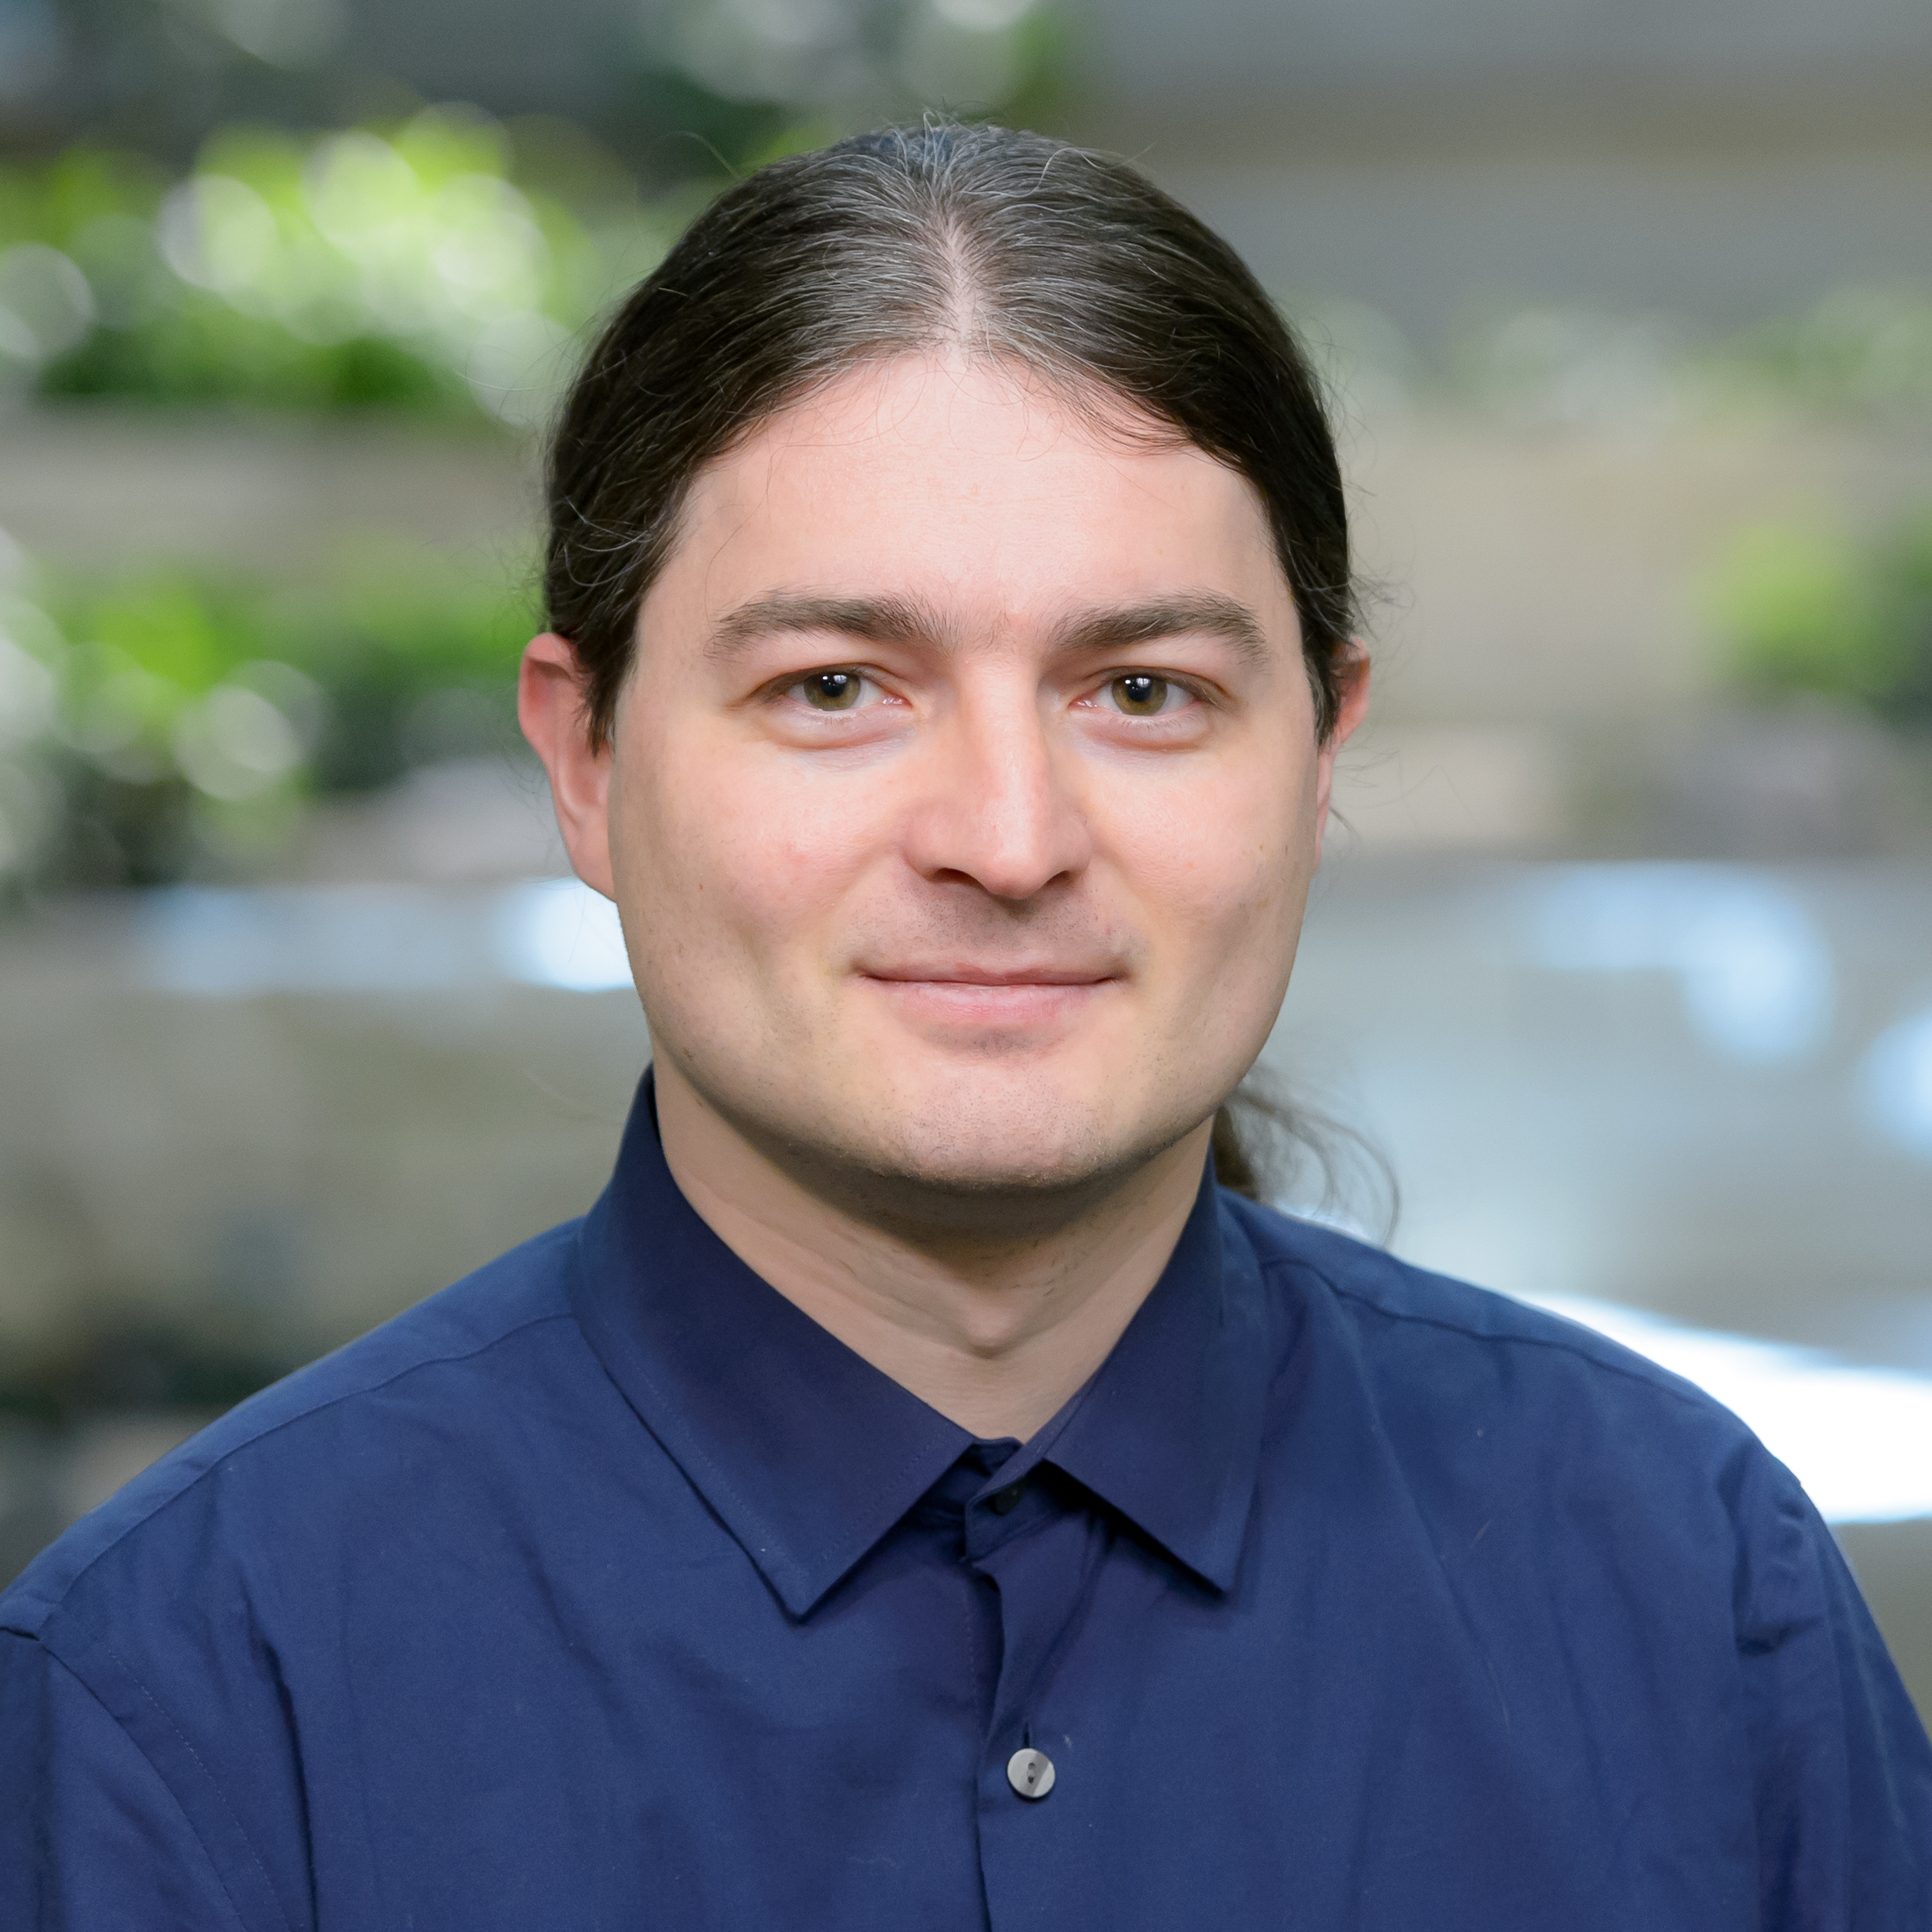
\includegraphics[width=\linewidth]{figs/portrait}
\end{column}
\begin{column}[c]{0.58\textwidth}
\begin{itemize}
\item At AMD since 2024
\item Working on 
  \begin{itemize}
  \item Fortran
  \item OpenMP
  \item GPGPU Offloading
  \item Loops
  \end{itemize}
 \item Converted Flang's runtime to use the \shinline{LLVM_ENABLE_RUNTIMES} system\itemremark{
    \begin{minipage}{\linewidth}
    \begin{tightcenter}
    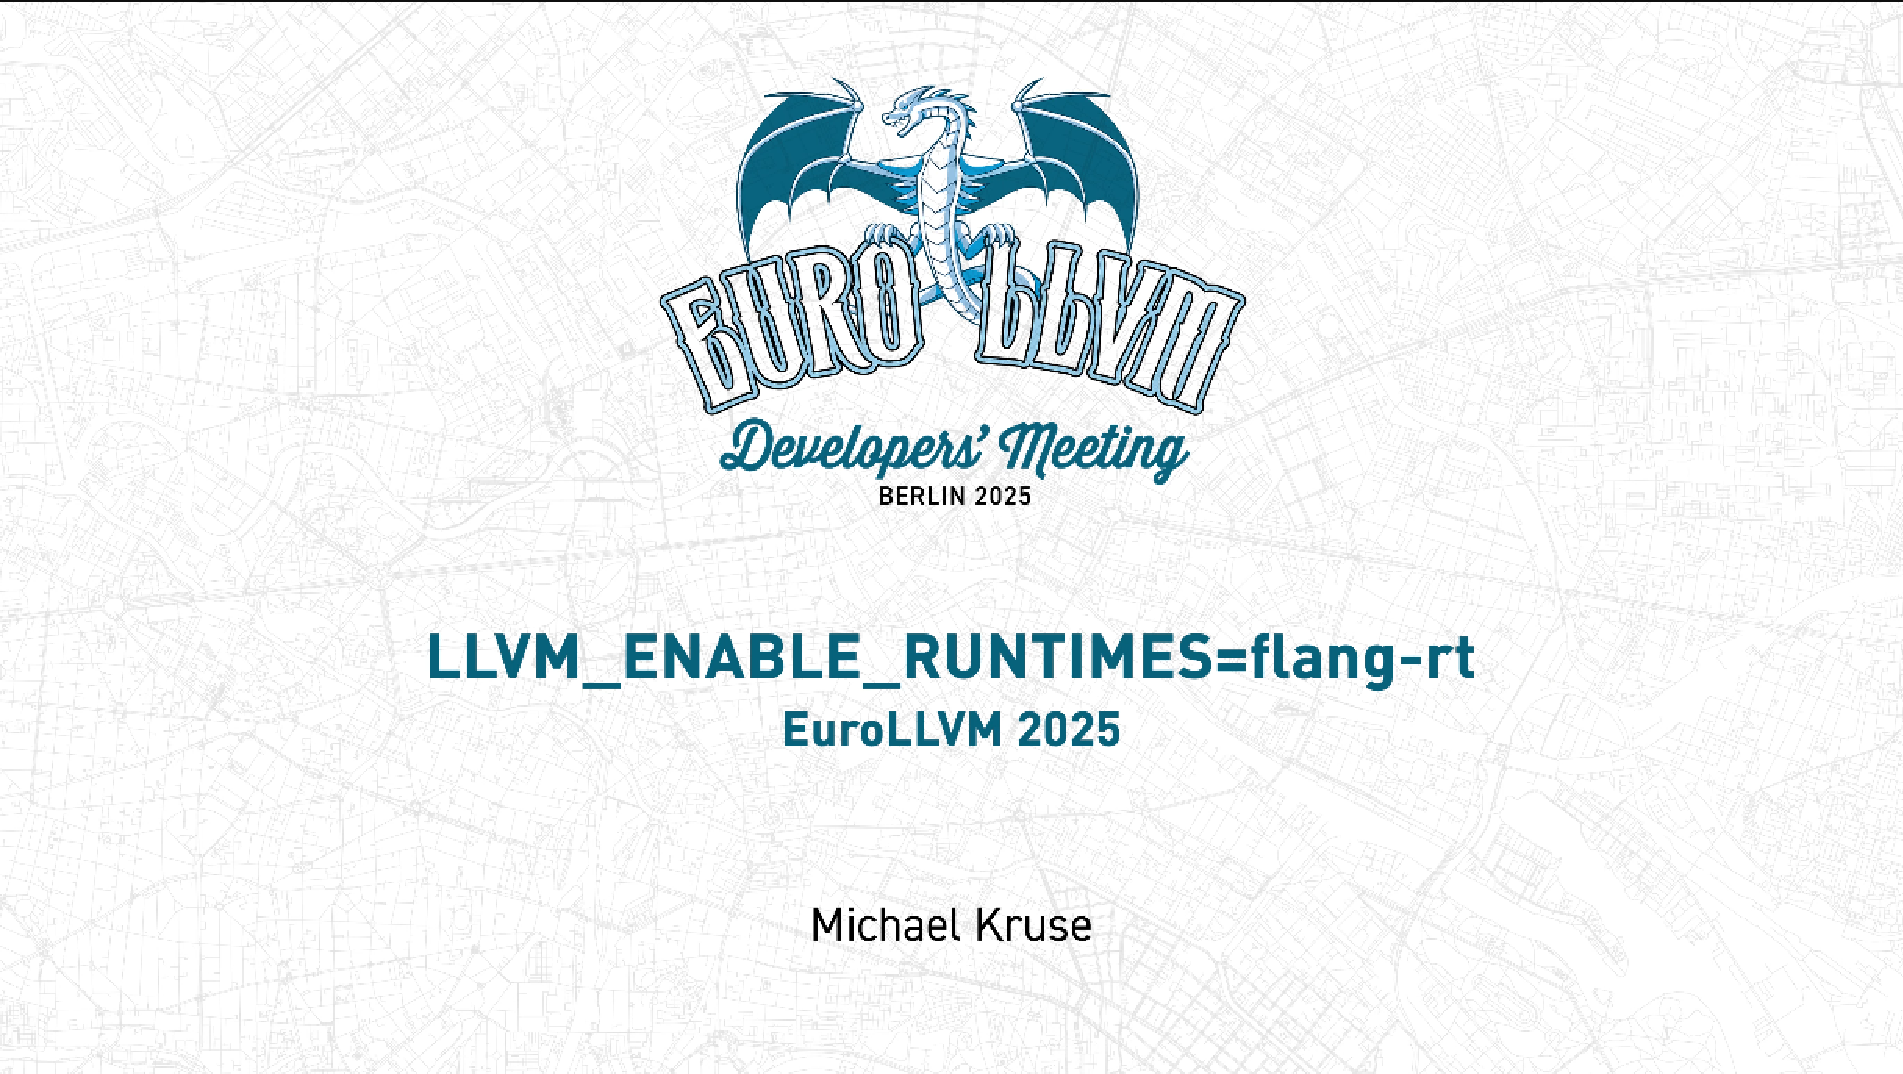
\includegraphics[width=0.7\linewidth]{figs/eurollvm2025talk}\\
    \url{https://youtu.be/AGrInJLxJ0Q}
    \end{tightcenter}
    \end{minipage}
 }
\end{itemize}
\end{column}
\end{columns}

\end{frame}




%%%%%%%%%%%%%%%%%%%%%%%%%%%%%%%%%%%%%%%%%%%%%%%%%%%%%%%%%%%%%%%%%%%%%%%%%%%%%%%%
\subsection{Why This Tutorial?}

\begin{frame}[fragile]{Why This Tutorial}

\begin{locate}<1->[anchor=center]{page cs:x=0.5,y=0.5}
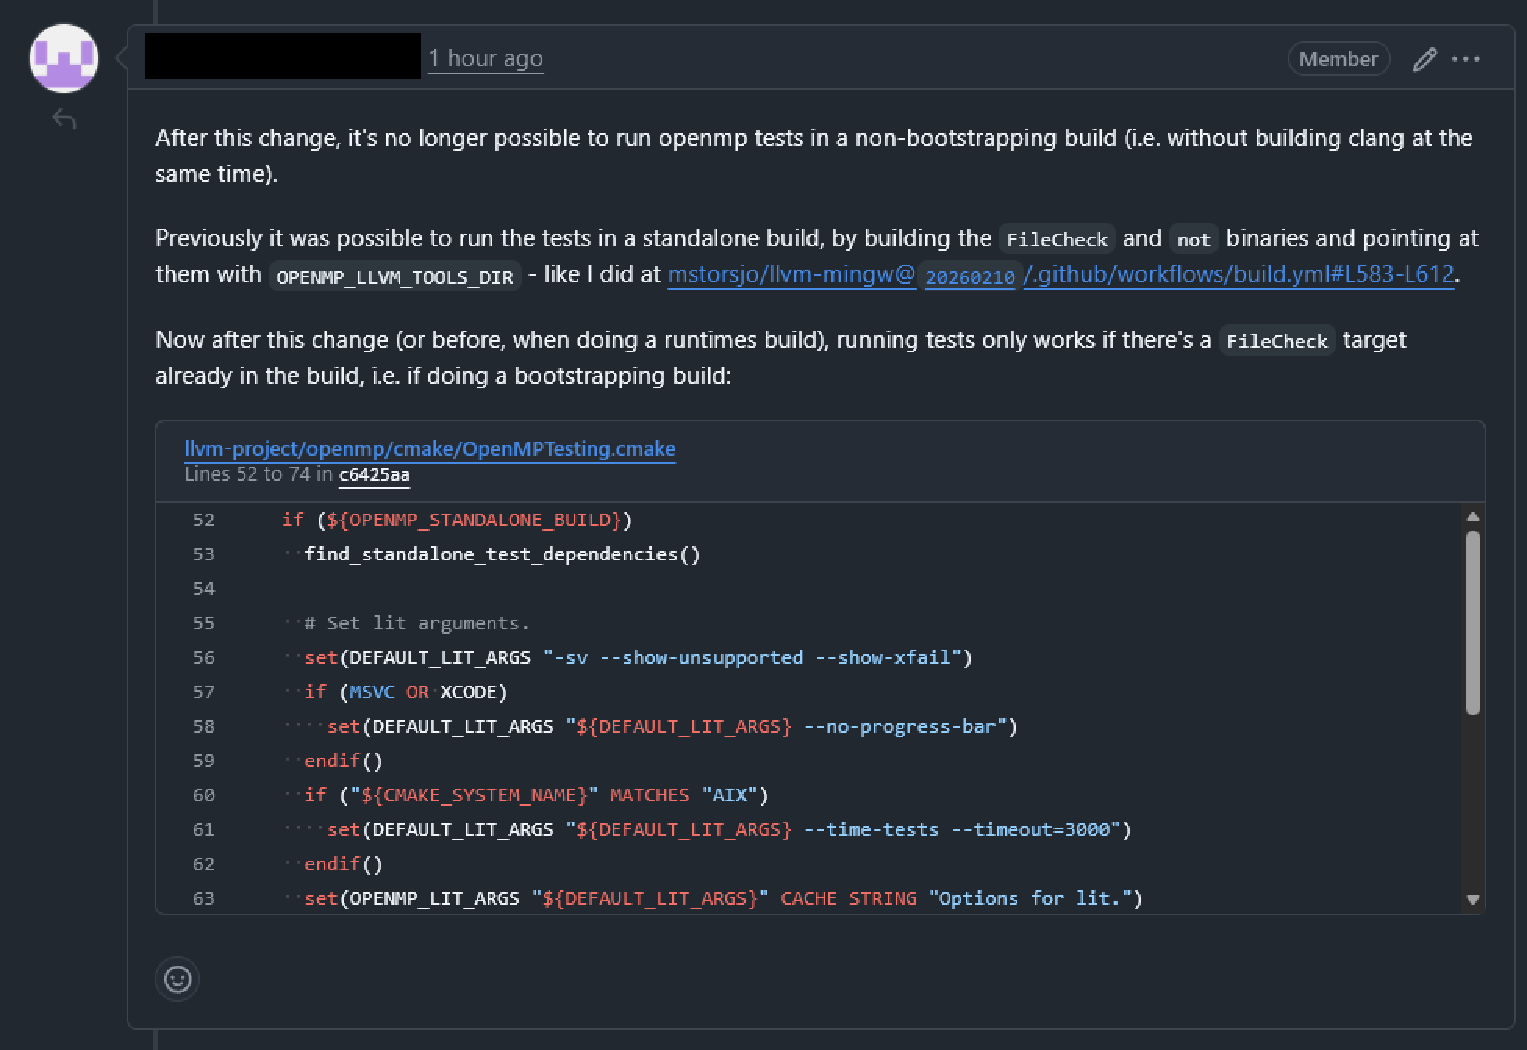
\includegraphics[width=0.6\pagewidth]{figs/ignorance1.pdf}
\end{locate}

\begin{locate}<2->[anchor=center,rotate=2]{page cs:x=0.5,y=0.5}
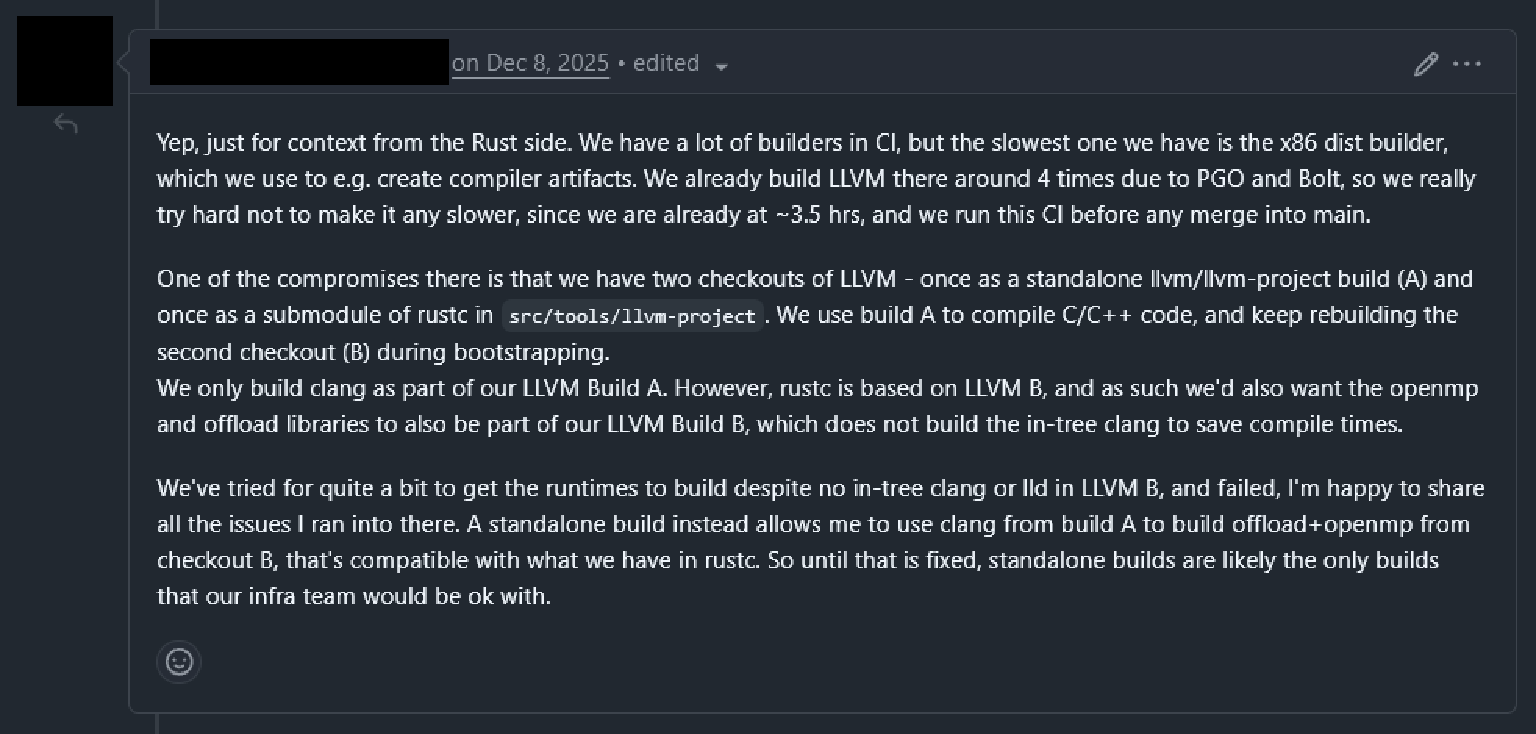
\includegraphics[width=0.8\pagewidth]{figs/ignorance2.pdf}
\end{locate}

\begin{locate}<3->[anchor=center,rotate=4]{page cs:x=0.5,y=0.6}
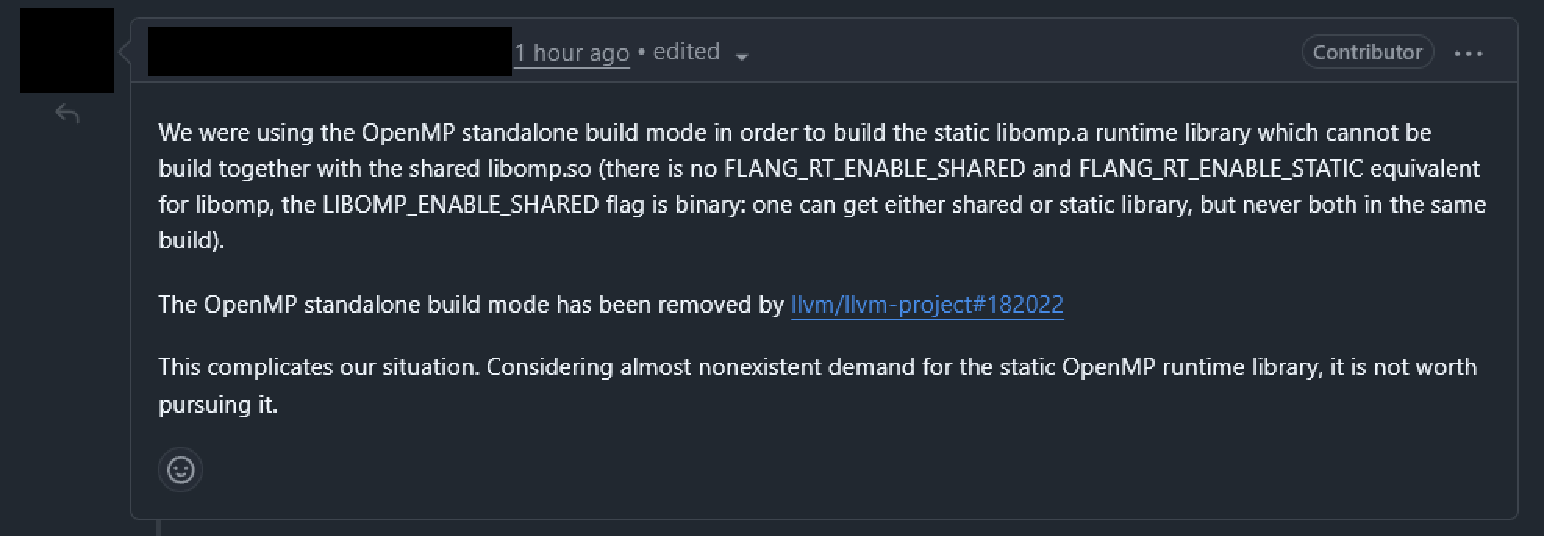
\includegraphics[width=0.7\pagewidth]{figs/ignorance3}
\end{locate}

\begin{locate}<4->[anchor=center,rotate=6]{page cs:x=0.6,y=0.5}
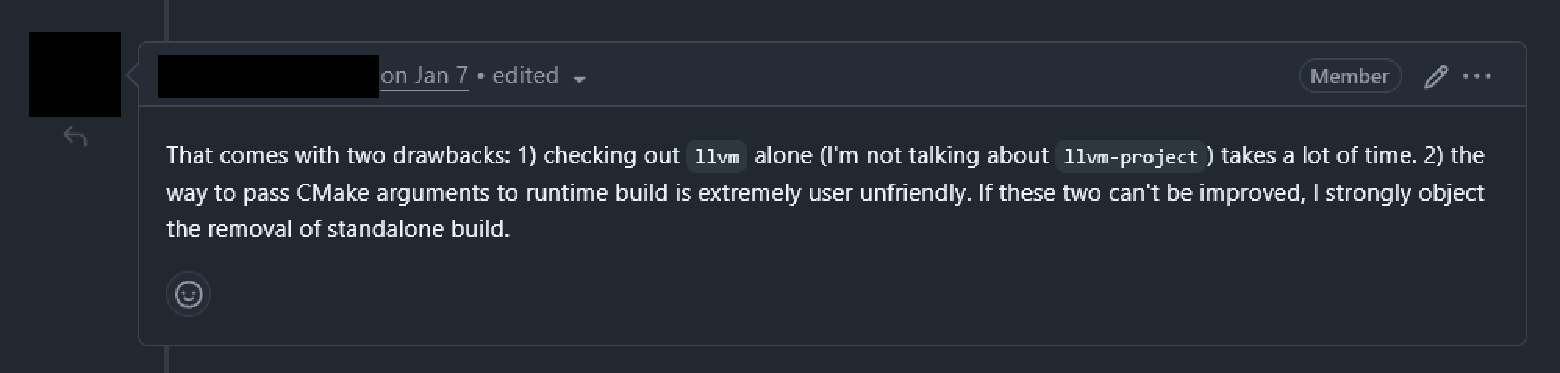
\includegraphics[width=0.7\pagewidth]{figs/ignorance4}
\end{locate}

\begin{locate}<5->[anchor=center,rotate=8]{page cs:x=0.5,y=0.4}
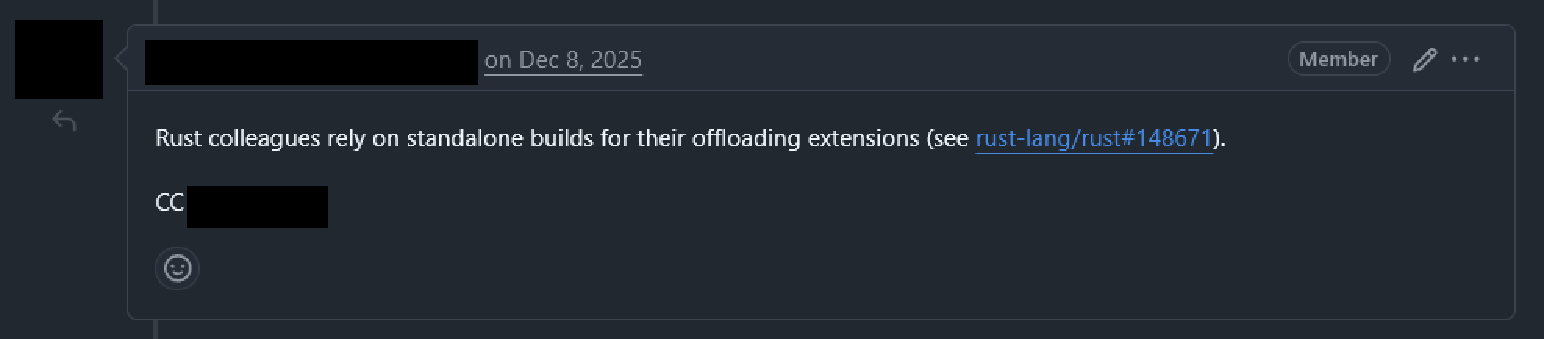
\includegraphics[width=0.7\pagewidth]{figs/ignorance5}
\end{locate}

\begin{locate}<6->[anchor=center,rotate=10]{page cs:x=0.4,y=0.5}

\includegraphics[width=0.7\pagewidth]{figs/ignorance6}
\end{locate}

\begin{locate}<7->[anchor=center,rotate=-4]{page cs:x=0.5,y=0.5}

\includegraphics[width=0.8\pagewidth]{figs/ignorance7}
\end{locate}

\end{frame}






%%%%%%%%%%%%%%%%%%%%%%%%%%%%%%%%%%%%%%%%%%%%%%%%%%%%%%%%%%%%%%%%%%%%%%%%%%%%%%%%
\subsection{History}

\begin{frame}[fragile]{History}
\begin{enumerate}
\item<1-> Initially, each subproject had its own SVN repository
  \begin{itemize}
  \item Subprojects categorized as \dquote{tools} (clang: 2009), \dquote{runtime} (libprofile), and \dquote{projects} (e.g., llvm-gcc)
  \item An example project boilerplate existed
   %\footnote{\url{https://github.com/llvm/llvm-project/tree/afbe97542f6fbf2b0dac0ede5e8a38ff0b9f24c7/llvm/projects/sample}}
  \end{itemize}
\item<2-> \dquote{runtime} subdirectory disappears with dysfunct PGO removal (2013)
 
\item<3-> Desire to separate runtimes\footnote{\url{https://reviews.llvm.org/D20992}}\footnote{%Original proposal:
 \url{https://lists.llvm.org/pipermail/llvm-dev/2020-October/145997.html}} (2016--2020)
  \begin{itemize}
  \item Somewhat different from compile-time utils/tools/compilers
  \end{itemize}
  
\item<4-> Introduction of \textinline{LLVM_ENABLE_PROJECTS}\footnote{\url{https://reviews.llvm.org/D26365}} (2016)
\item<4-> Introduction of \textinline{LLVM_ENABLE_RUNTIMES}\footnote{\url{https://reviews.llvm.org/D132478}} (2022)
  \begin{itemize}
  \item First for libc++
  \end{itemize}
\end{enumerate}
\end{frame}



%%%%%%%%%%%%%%%%%%%%%%%%%%%%%%%%%%%%%%%%%%%%%%%%%%%%%%%%%%%%%%%%%%%%%%%%%%%%%%%%
\begin{comment}
%\subsection{CMake Basics}
%
%\begin{frame}[fragile]{CMake Basics}
%\begin{itemize}[<+->]
%\item Do not use \textinline{set(VAR_NAME)}
%\item Do not use \textinline{if (${VAR_NAME})}
%\end{itemize}
%\end{frame}
\end{comment}



%%%%%%%%%%%%%%%%%%%%%%%%%%%%%%%%%%%%%%%%%%%%%%%%%%%%%%%%%%%%%%%%%%%%%%%%%%%%%%%%
\subsection{Rationale}
\begin{frame}[fragile,shrink=10]{Rationale}
\framesubtitle{Why \textinline{LLVM_ENABLE_RUNTIMES}?}

\begin{columns}[t]
\begin{column}{0.31\textwidth}
\anchor[t]{anw}%
\begin{block}{Build Host}
The system we build on
\begin{itemize}
\item \shinline{cmake}, \shinline{ninja}, \shinline{cc}, \dots
\item \shinline{llvm-tblgen}, \shinline{mlir-tblgen}, \dots
\end{itemize}
\end{block}
\end{column}%
\begin{column}{0.31\textwidth}\anchor[t]{dummy}%
\begin{block}{Cross-Compile Target}
Where Clang will run
\begin{itemize}
\item \shinline{clang}, \shinline{opt}, \shinline{lld}, \dots
\item \shinline{LLVMSupport}\{\shinline{.a}/\shinline{.so}\},  \shinline{LLVMPolly.so}, \dots
\end{itemize}%
\end{block}\anchor[b]{asw}%
\end{column}\anchor[t]{ane}%
\begin{column}{0.31\textwidth}%
\anchor[t]{bnw}%
\begin{block}{Compiler Target}
What Clang will compile for
\begin{itemize}
\item \shinline{a.out}
\item compiler-rt, \shinline{libc}, \shinline{libc++}, \dots
\end{itemize}
\end{block}\anchor[b]{bsw}
\end{column}\anchor[t]{bne}
\end{columns}

\vspace{3ex}

\begin{itemize}
\item Automate multiple build-steps
\begin{itemize}
\item Instead of: Build clang \textrightarrow{} build compiler-rt for x86\_64 \textrightarrow{} build compiler-rt for arm64 \textrightarrow{} \dots
\end{itemize}
\item Reduce per-runtime boilerplate/differences between build modes
\item \alert<2->{Runtimes compiled (Stage 2) using just-built Clang}
\end{itemize}

\begin{tikzpicture}[overlay,remember picture]
\node<2->[rounded corners,draw=red,fit={(anw) (asw) (ane)},inner xsep=0,inner ysep=-1.5ex, xshift=-1.5mm](stage1) {};
\node<2->[below=0.5ex of stage1,text=red](stage) {Stage 1};

\node<2->[rounded corners,draw=red,fit={(bnw) (bsw) (bne)},inner xsep=0,inner ysep=-1.5ex, xshift=-1.5mm](stage2) {};
\node<2->[below=0.5ex of stage2,text=red](stage) {Stage 2};
\end{tikzpicture}

\end{frame}



%%%%%%%%%%%%%%%%%%%%%%%%%%%%%%%%%%%%%%%%%%%%%%%%%%%%%%%%%%%%%%%%%%%%%%%%%%%%%%%%
\subsection{Goal}
\begin{frame}[fragile]{Tutorial Runtime}
\framesubtitle{What is our tutorial runtime going to do?}

\begin{block}{Our Runtime}
\begin{minted}{c}
void _dublin_hello_world() {
  puts("Dia daoibh, a dhomhain!\n");
}
\end{minted}
\end{block}

\bigskip

\begin{itemize}
\item Use LLVM best-practices
\item Linux only
%  \begin{itemize}
%  \item No Windows/MacOS/AIX/\dots
%  \end{itemize}
\item Prioritize conciseness and principles over
\begin{itemize}
\item \dots{} features
\item \dots{} comments
\item \dots{} unrelated boilerplate
\end{itemize}
\item Point out shortcomings of the current system
\end{itemize}
\end{frame}



%%%%%%%%%%%%%%%%%%%%%%%%%%%%%%%%%%%%%%%%%%%%%%%%%%%%%%%%%%%%%%%%%%%%%%%%%%%%%%%%
%%%%%%%%%%%%%%%%%%%%%%%%%%%%%%%%%%%%%%%%%%%%%%%%%%%%%%%%%%%%%%%%%%%%%%%%%%%%%%%%
\section{Let's Create a Runtime}


%%%%%%%%%%%%%%%%%%%%%%%%%%%%%%%%%%%%%%%%%%%%%%%%%%%%%%%%%%%%%%%%%%%%%%%%%%%%%%%%
\subsection{Setup}
\begin{frame}[fragile]{Setup}
\framesubtitle{\url{https://github.com/Meinersbur/llvm-dublin/tree/dublin-0-main}}
\begin{itemize}
\item[\pgfuseimage{file}] \shinline{README.md}
  \begin{itemize}
  \item Update Readme for tutorial
  \end{itemize}
\item[\pgfuseimage{file}] \shinline{.gitignore}
  \begin{itemize}
  \item Make git ignore \textinline{install*} subdirs \itemremark{(like \textinline{build*} already is)}
  \end{itemize}
\end{itemize}

\medskip

\begin{block}{\shinline{$HOME/bin/cmake}}
\begin{minted}{sh}
/usr/bin/cmake -G Ninja                               \
               -D CMAKE_C_COMPILER_LAUNCHER=ccache    \
               -D CMAKE_CXX_COMPILER_LAUNCHER=ccache  \
               -D CMAKE_DISABLE_PRECOMPILE_HEADERS=ON \
               "$@"
\end{minted}
\end{block}
\end{frame}



%%%%%%%%%%%%%%%%%%%%%%%%%%%%%%%%%%%%%%%%%%%%%%%%%%%%%%%%%%%%%%%%%%%%%%%%%%%%%%%%
\subsection{Step 1: Register with the LLVM Build System}
\begin{frame}[fragile]{Register with the LLVM Build System}
\framesubtitle{\url{https://github.com/Meinersbur/llvm-dublin/tree/dublin-1-basic}}
\begin{itemize}
  \item[\pgfuseimage{file}] \shinline{llvm/CMakeLists.txt}
  \item[\pgfuseimage{file}] \shinline{runtimes/CMakeLists.txt}
  \begin{itemize}
      \item Allow \shinline{LLVM_ENABLE_RUNTIME=dublin}
  \end{itemize}

  \item[\pgfuseimage{file}] \shinline{dublin/CMakeLists.txt}
  \item[\pgfuseimage{file}] \shinline{dublin/CODE_OWNERS.TXT}
  \item[\pgfuseimage{file}] \shinline{dublin/LICENSE.TXT}
  \begin{itemize}
    \item Subproject boilerplate
  \end{itemize}
\end{itemize}
\end{frame}



%%%%%%%%%%%%%%%%%%%%%%%%%%%%%%%%%%%%%%%%%%%%%%%%%%%%%%%%%%%%%%%%%%%%%%%%%%%%%%%%
\subsection{Step 2: Build a Library Artifact}
\begin{frame}[fragile]{Step 2: Build a Library Artifact}
\begin{itemize}
\item[\pgfuseimage{file}] \shinline{lib/Dublin/dublin.c}
\item[\pgfuseimage{file}] \shinline{include/dublin/Dublin/dublin.h}
  \begin{itemize}
    \item Library sources
  \end{itemize}

\item[\pgfuseimage{file}] \shinline{lib/Dublin/CMakeLists.txt}
  \begin{itemize}
    \item Build instructions for \shinline{libdublin.a}
  \end{itemize}
\end{itemize}
\end{frame}



%%%%%%%%%%%%%%%%%%%%%%%%%%%%%%%%%%%%%%%%%%%%%%%%%%%%%%%%%%%%%%%%%%%%%%%%%%%%%%%%
\forestset{dirtree/.style={s sep=1mm,font=\footnotesize,
    font=\ttfamily,
    grow'=0,
    child anchor=west,
    parent anchor=south,
    anchor=west,
    calign=first,
    edge path={
      \noexpand\path [draw, \forestoption{edge}]
      (!u.south west) +(7.5pt,0) |- node[fill,inner sep=1.25pt] {} (.child anchor)\forestoption{edge label};
    },
    before typesetting nodes={
      if n=1
        {insert before={[,phantom]}}
        {}
    },
    fit=band,
    before computing xy={l=15pt},
    }}


\begin{frame}[fragile]{Standard Subproject Layout}
\begin{scaleenv}{0.6}
\begin{columns}[t]
\begin{column}[t]{0.5\textheight}
\begin{forest}
for tree={dirtree}
[subproject, font=\sffamily
  [docs
    [{*.rst, *.md}]
  ]
  [examples
    [Example1
      [{*.c, *.cpp}]
    ]
  ]
  [test
    [Unit
      [{lit.cfg.py, lit.site.cfg.py.in}]
    ]
    [Component1, font=\sffamily
      [{*}]
    ]
    [Component2, font=\sffamily
      [{*}]
    ]
    [{lit.cfg.py, lit.site.cfg.py.in}]
  ]
  [unittests
    [Component1, font=\sffamily
      [Component1Test.cpp]
    ]
    [Component2, font=\sffamily
      [Component1Test.cpp]
    ]
  ]
]
\end{forest}
\end{column}
\begin{column}[t]{0.5\textheight}
\begin{forest}
for tree={dirtree}
[
  [cmake
    [Modules/modules
      [*.cmake]
    ]
    [caches
      [*.cmake]
    ]
  ]
  [include
    [subproject, font=\sffamily
      [Component1, font=\sffamily
        [component1.h]
      ]
      [Component2, font=\sffamily
        [component2.h]
      ]
    ]
  ]
  [lib
    [Component1, font=\sffamily
      [component1.c]
      [component1-internal.h]
    ]
    [Component2, font=\sffamily
      [component2.c]
    ]
  ]
  [utils
    [utility, font=\sffamily
      [utility.cpp]
    ]
  ]
]
\end{forest}
\end{column}
\end{columns}
\end{scaleenv}
\end{frame}



%%%%%%%%%%%%%%%%%%%%%%%%%%%%%%%%%%%%%%%%%%%%%%%%%%%%%%%%%%%%%%%%%%%%%%%%%%%%%%%%
\subsection{Step 3: An Example that uses the Library}
\begin{frame}[fragile]{An Example that uses the Library}
\framesubtitle{\url{https://github.com/Meinersbur/llvm-dublin/tree/dublin-3-example}}
\begin{itemize}
\item[\pgfuseimage{file}] \shinline{examples/dublin-hello/dublin-hello.c}
  \begin{itemize}
  \item Example source
  \end{itemize}
\item[\pgfuseimage{file}] \shinline{examples/dublin-hello/CMakeLists.txt}
  \begin{itemize}
  \item Example build instructions
  \end{itemize}
\end{itemize}
\end{frame}



%%%%%%%%%%%%%%%%%%%%%%%%%%%%%%%%%%%%%%%%%%%%%%%%%%%%%%%%%%%%%%%%%%%%%%%%%%%%%%%%
\begin{frame}[fragile]{Common What To Build Options}
\begin{itemize}
\item \textinline{DUBLIN_INCLUDE_<component>}
  \begin{itemize}
  \item Executes \textinline{add_subdirectory(<component>)}
  \item \textinline{ninja <component>} can be used
  \item Default to \textinline{LLVM_INCLUDE_<component>}
  \end{itemize}
\item[]
\item \textinline{DUBLIN_BUILD_<component>}
  \begin{itemize}
  \item \textinline{ninja all} also builds \textinline{<component>} 
  \item Generally steers which target use \textinline{ALL}/\textinline{EXCLUDE_FROM_ALL}
  \item Default to \textinline{LLVM_BUILD_<component>}
  \end{itemize}
\end{itemize}
\end{frame}



%%%%%%%%%%%%%%%%%%%%%%%%%%%%%%%%%%%%%%%%%%%%%%%%%%%%%%%%%%%%%%%%%%%%%%%%%%%%%%%%
\subsection{Step 4: Build Modes}
\framesubtitle{\url{https://github.com/Meinersbur/llvm-dublin/tree/dublin-4-modes}}
\begin{frame}[fragile]{Build Modes}
\begin{itemize}
  \item[\pgfuseimage{file}] \shinline{CMakeLists.txt}
  \begin{itemize}
     \item Detect unsupported legacy build modes
  \end{itemize}
\end{itemize}
\end{frame}



%%%%%%%%%%%%%%%%%%%%%%%%%%%%%%%%%%%%%%%%%%%%%%%%%%%%%%%%%%%%%%%%%%%%%%%%%%%%%%%%
\begin{frame}[fragile,shrink=20]{Build Modes}

%\begin{columns}[t]
%\begin{column}{0.48\textwidth}
%
%\end{column}
%\begin{column}{0.48\textwidth}
%
%\end{column}
%\end{columns}


\vspace*{3ex}

\begin{block}{Legacy Build Modes}
%\begin{itemize}
%\item Standalone: \shinline{cmake -S dublin}
%\item As Project: \shinline{cmake -S llvm -DLLVM_ENABLE_PROJECTS=dublin}
%\end{itemize}
\begin{tabular}{llll}
\textbf{As project:} & \shinline{cmake} & \shinline{-S <llvm-project>/llvm}   & \shinline{-D LLVM_ENABLE_PROJECTS=dublin}\\
\textbf{Standalone:} & \shinline{cmake} & \shinline{-S <llvm-project>/dublin} & \\
\end{tabular}
\medskip
\begin{itemize}
\item Intended to be superseded by runtimes build modes\footnote{\url{https://lists.llvm.org/pipermail/llvm-dev/2020-October/145997.html}}
\item If your build infrastructure still uses this, please consider updating
\item Even \dquote{standalone} mode needs files from sibling directories
  \itemremark{A consequence of the monorepository}
\end{itemize}
\end{block}


\begin{block}{Runtimes Build Modes}
%\begin{itemize}
%\item Bootstrapping:      \shinline{cmake -S llvm -DLLVM_ENABLE_RUNTIMES=dublin}
%\item Default/Standalone: \shinline{cmake -S runtimes -DLLVM_ENABLE_RUNTIMES=dublin}
%\end{itemize}
\begin{tabular}{llll}
\textbf{Bootstrapping:}      & \shinline{cmake} & \shinline{-S <llvm-project>/llvm} & \shinline{-D LLVM_ENABLE_RUNTIMES=dublin}\\
\textbf{Default/Standalone:} & \shinline{cmake} & \shinline{-S <llvm-project>/runtimes} & \shinline{-D LLVM_ENABLE_RUNTIMES=dublin}\\
\end{tabular}
\medskip
\begin{itemize}
\item Shared boilerplate code in \shinline{<llvm-project>/runtimes/CMakeLists.txt}
\end{itemize}
\end{block}

% Build Modes: \url{https://github.com/llvm/llvm-project/pull/170693#issuecomment-3720262808}
\end{frame}




%%%%%%%%%%%%%%%%%%%%%%%%%%%%%%%%%%%%%%%%%%%%%%%%%%%%%%%%%%%%%%%%%%%%%%%%%%%%%%%%
\begin{frame}[fragile]{Bootstrapping Runtimes Build Mode}

\begin{tightcenter}
% https://sequencediagram.org/
% Inkscape: remove background & export pdf
% gswin64 -o bootstrapping-inverted.pdf -sDEVICE=pdfwrite -c "{1 exch sub}{1 exch sub}{1 exch sub}{1 exch sub} setcolortransfer" -f bootstrapping.pdf
\begin{comment}
actor User
participant "build/" as build
participant "build/runtimes/runtimes-bins/" as runtimes

User->build:cmake -S <llvm-project>/llvm\n  -D LLVM_ENABLE_RUNTIMES=dublin\n  ...
activate build
space -1
deactivate build
#build->runtimes:create

User->build:ninja configure-runtimes
activate build
space -3
build->build:ninja clang FileCheck not ...
build->runtimes:cmake -S <llvm-project>/runtimes\n  -D CMAKE_C_COMPILER=clang\n  -D LLVM_BINARY_DIR=build/\n  -D LLVM_ENABLE_RUNTIMES=dublin\n  ...
activate runtimes
space -1
deactivate runtimes
deactivate build

User->build:ninja dublin
activate build
build->runtimes:ninja dublin
activate runtimes
space 
deactivate runtimes
deactivate build
\end{comment}
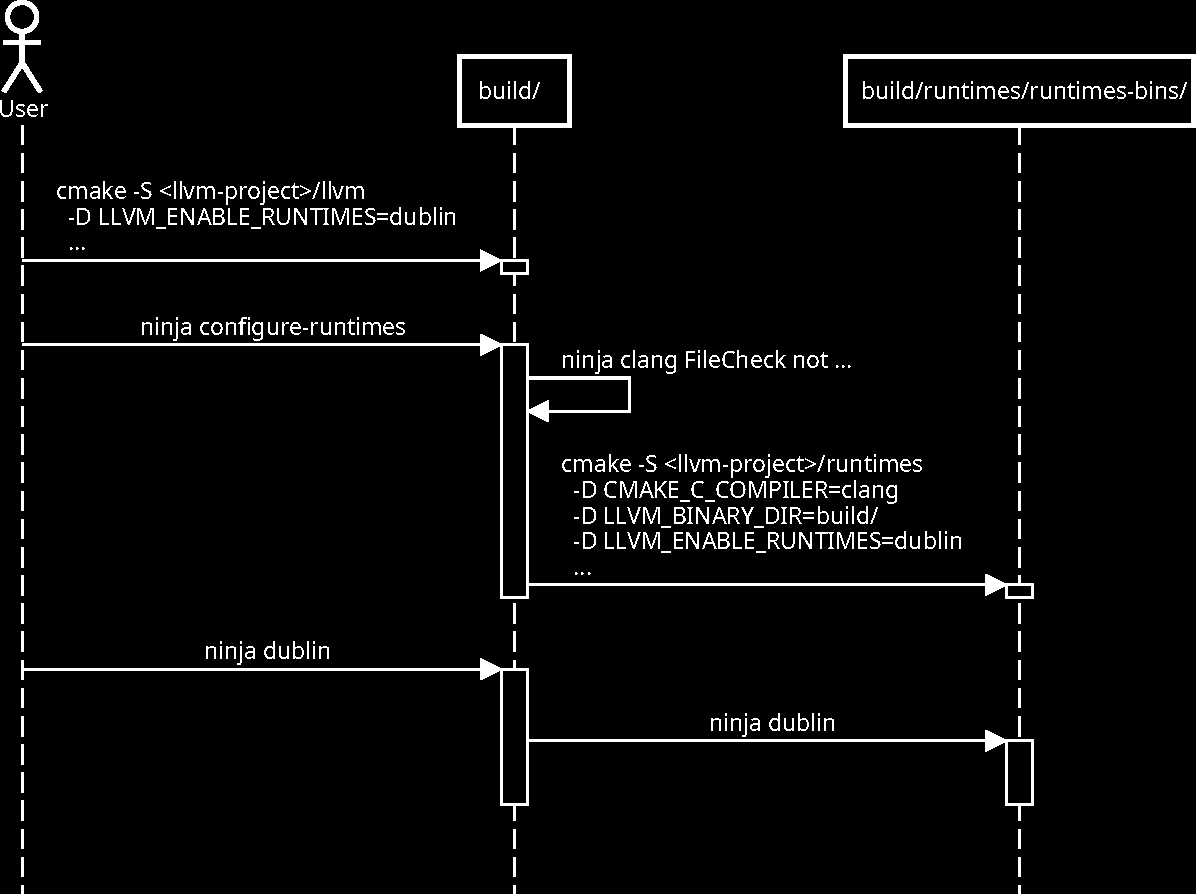
\includegraphics[height=0.9\pageheight]{figs/bootstrapping-inverted}
\end{tightcenter}

\end{frame}



%%%%%%%%%%%%%%%%%%%%%%%%%%%%%%%%%%%%%%%%%%%%%%%%%%%%%%%%%%%%%%%%%%%%%%%%%%%%%%%%
\begin{frame}[fragile]{Default/Standalone Runtimes Build Mode}
\framesubtitle{Skip the Middleman}

\begin{tightcenter}
% Invert pdf using:
% gswin64 -o standalone-inverted.pdf -sDEVICE=pdfwrite -c "{1 exch sub}{1 exch sub}{1 exch sub}{1 exch sub} setcolortransfer" -f standalone.pdf
\begin{comment}
actor User
participant "build-runtimes/" as runtimes

User->runtimes:cmake -S <llvm-project>/runtimes\n  -D CMAKE_C_COMPILER=clang\n  -D LLVM_BINARY_DIR=build/\n  -D LLVM_ENABLE_RUNTIMES=dublin\n  ...
activate runtimes
space -1
deactivate runtimes

User->runtimes:ninja dublin
activate runtimes
space
deactivate runtimes
\end{comment}
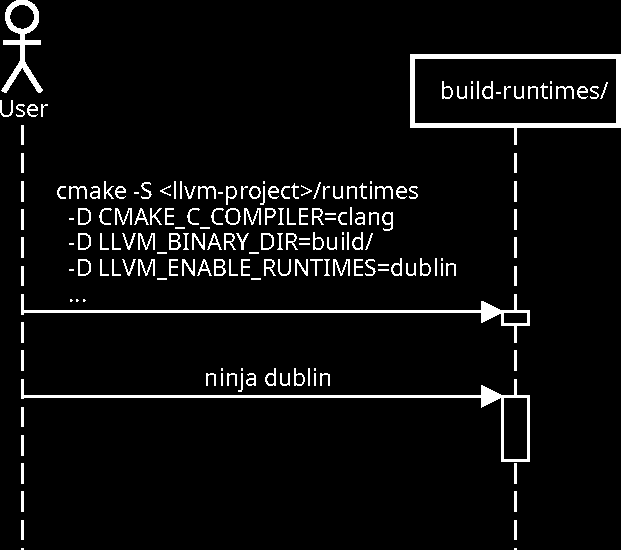
\includegraphics[height=0.6\pageheight]{figs/standalone-inverted}
\end{tightcenter}
\end{frame}


%%%%%%%%%%%%%%%%%%%%%%%%%%%%%%%%%%%%%%%%%%%%%%%%%%%%%%%%%%%%%%%%%%%%%%%%%%%%%%%%
\begin{frame}[fragile]{Default/Standalone Runtimes Build Mode}

\begin{block}{\shinline{runtimes/CMakeLists.txt}}
\begin{minted}{cmake}
project(Runtimes C CXX ASM)

find_package(LLVM HINT ${LLVM_BINARY_DIR})
# more boilerplate code

foreach (runtime ${LLVM_ENABLE_RUNTIMES})
  add_subdirectory(${runtime})
endforeach ()
\end{minted}
\end{block}



\end{frame}


%%%%%%%%%%%%%%%%%%%%%%%%%%%%%%%%%%%%%%%%%%%%%%%%%%%%%%%%%%%%%%%%%%%%%%%%%%%%%%%%
\begin{comment}
\begin{frame}[fragile,shrink=5]{Bootstrapping Build Mode}

\begin{block}{\shinline{llvm/runtimes/CMakeLists.txt}}
\begin{itemize}
\item Configure nested builddirs
  \begin{itemize}
  \item \shinline{runtimes/buitins-bins} for Compiler-RT
  \item \shinline{runtimes/runtimes-bins}
  \end{itemize}
\item Forward configuration parameters
  \begin{itemize}
  \item Selected configuration options (e.g., \shinline{LLVM_INCLUDE_TESTS})
  \item Any option that starts with the capitalized runtime name (i.e., \textinline{DUBLIN_*})
  \item The content of \textinline{RUNTIMES_CMAKE_ARGS}\itemremark{e.g., \shinline{-DRUNTIMES_CMAKE_ARGS="-DCMAKE_CXX_FLAGS=-ferror-limit=1"}}
  \end{itemize}
\item Build prerequisites
  \begin{itemize}
  \item Test infrastructure: \shinline{llvm-lit}, \shinline{FileCheck}, \shinline{not}, \dots
  \item Compilers: Clang, Flang (if enabled via \textinline{CMAKE_ENABLE_PROJECTS})
  \end{itemize}
\item Build targets for the nested builddir(s)
  \begin{itemize}
  \item Control targets: \shinline{configure-runtimes}, \shinline{install-runtimes}, \shinline{clean-runtimes}, \dots
  \item Added dependency: \shinline{all}, \shinline{install}
  \item Just forwarded: \shinline{dublin}, \shinline{check-dublin}, \shinline{runtimes} \textrightarrow{} \shinline{all}
  \end{itemize}
\end{itemize}
\end{block}
\end{frame}
\end{comment}


%%%%%%%%%%%%%%%%%%%%%%%%%%%%%%%%%%%%%%%%%%%%%%%%%%%%%%%%%%%%%%%%%%%%%%%%%%%%%%%%
\subsection{Step 5: CMake Cache Files}
\begin{frame}[fragile]{CMake Cache Files}
\framesubtitle{\url{https://github.com/Meinersbur/llvm-dublin/tree/dublin-5-cachefiles}}
\begin{itemize}
\item[\pgfuseimage{file}] \shinline{cmake/caches/runtimes-bins.cmake}
  \begin{itemize}
  \item Pre-populated CMake parameters as a bootstrapping build would set them
  \end{itemize}
\end{itemize}
\end{frame}



%%%%%%%%%%%%%%%%%%%%%%%%%%%%%%%%%%%%%%%%%%%%%%%%%%%%%%%%%%%%%%%%%%%%%%%%%%%%%%%%
\subsection{Step 6: Artifact Output Location}
\begin{frame}[fragile]{Artifact Output Location}
\framesubtitle{\url{https://github.com/Meinersbur/llvm-dublin/tree/dublin-6-location}}
\begin{itemize}
\item[\pgfuseimage{file}] \shinline{CMakeLists.txt}, \shinline{cmake/Modules/GetToolchainDirs.cmake}
  \begin{itemize}
  \item Determine standard locations 
  \end{itemize}
\item[\pgfuseimage{file}] \shinline{lib/Dublin/CMakeLists.txt}
  \begin{itemize}
  \item Set artifact output location
  \end{itemize}
\end{itemize}
\end{frame}


%%%%%%%%%%%%%%%%%%%%%%%%%%%%%%%%%%%%%%%%%%%%%%%%%%%%%%%%%%%%%%%%%%%%%%%%%%%%%%%%
\begin{frame}[fragile]{Library Locations}
\framesubtitle{\shinline{LLVM_ENABLE_PER_TARGET_RUNTIME_DIR=ON}}
%\begin{scaleenv}{0.6}
\vspace*{-\baselineskip}
\begin{columns}[t]
\begin{column}[t]{0.48\textwidth}
\begin{block}{Installation Prefix Dir}
\begin{minipage}[t][48mm][t]{\textwidth}
\begin{tightcenter}
\begin{forest}
for tree={dirtree}
[{\$PREFIX}
  [bin
    [clang]
  ]
  [lib
    [<target triple>, font=\sffamily
      [{*.so, *.a}]
    ]
  ]
]
\end{forest}
\end{tightcenter}
\end{minipage}
\begin{itemize}
\item Accessible to any compiler when installed (including e.g., gcc)
\end{itemize}
\end{block}
\end{column}
\begin{column}[t]{0.48\textwidth}
\begin{block}{Resource Dir}
%\begin{minipage}[t][20mm][t]{\textwidth}
\begin{tightcenter}
\begin{forest}
for tree={dirtree}
[{\$PREFIX}
  [bin
    [clang]
  ]
  [lib
    [clang
      [<llvm version>, font=\sffamily
        [lib
          [<target triple>, font=\sffamily
            [{*.a}]
          ]
        ]
      ]
    ]
  ]
]
\end{forest}
\end{tightcenter}
%\vspace*{-30mm}
%\end{minipage}
\begin{itemize}
\item Accessible to only this version of Clang (and Flang)
\end{itemize}
\end{block}
\end{column}
\end{columns}
%\end{scaleenv}
\end{frame}



%%%%%%%%%%%%%%%%%%%%%%%%%%%%%%%%%%%%%%%%%%%%%%%%%%%%%%%%%%%%%%%%%%%%%%%%%%%%%%%%
\subsection{Step 7: Installation}
\begin{frame}[fragile]{Installation}
\framesubtitle{\url{https://github.com/Meinersbur/llvm-dublin/tree/dublin-7-install}}
\begin{itemize}
\item[\pgfuseimage{file}] \shinline{CMakeLists.txt}
  \begin{itemize}
  \item Set install output location
  \end{itemize}
\item[\pgfuseimage{file}] \shinline{lib/Dublin/CMakeLists.txt}
  \begin{itemize}
  \item Library installation
  \end{itemize}
\item[\pgfuseimage{file}] \shinline{include/CMakeLists.txt}
  \begin{itemize}
  \item Header installation
  \end{itemize}
\end{itemize}
\end{frame}



%%%%%%%%%%%%%%%%%%%%%%%%%%%%%%%%%%%%%%%%%%%%%%%%%%%%%%%%%%%%%%%%%%%%%%%%%%%%%%%%
\subsection{Step 8: Shared and Static Libraries}
\begin{frame}[fragile]{Shared and Static Libraries}
\framesubtitle{\url{https://github.com/Meinersbur/llvm-dublin/tree/dublin-8-shared}}
\begin{itemize}
\item[\pgfuseimage{file}] \shinline{cmake/Modules/AddDublin.cmake}
  \begin{itemize}
  \item If building Shared and Static library, use an OBJECT library
  \item Wrapper around CMake's native \textinline{add_library}
  \item \shinline{AddLLVM}'s \textinline{llvm_add_library} main service is linking to LLVM libraries
    \itemremark{Target triple confusion. Do not use.}
  \end{itemize}
\item[\pgfuseimage{file}] \shinline{lib/Dublin/CMakeLists.txt}
  \begin{itemize}
  \item Use \shinline{AddDublin.cmake} instead of \textinline{add_library}
  \end{itemize}
\end{itemize}
\end{frame}



%%%%%%%%%%%%%%%%%%%%%%%%%%%%%%%%%%%%%%%%%%%%%%%%%%%%%%%%%%%%%%%%%%%%%%%%%%%%%%%%
\begin{frame}[fragile,shrink=20]{OBJECT Libraries}
\begin{tightcenter}
\begin{tikzpicture}
\tikzset{node/.style={draw=teal,line width=1.2pt,rounded corners,top color=teal!50,bottom color=white,shading angle=15,blur shadow}}
\tikzset{edge/.style={->}}


\tikzset{supernode/.style={subgraph text none,draw=white,rounded corners}}
\tikzset{filenode/.style={minimum width=7mm,minimum height=1cm,align=flush left,grow=right,draw,shape=file,fill=white}}

\graph[layered layout,edges={edge,rounded corners},level sep=70mm,sibling sep=40mm,grow=right]{
%
objectlib [subgraph text none] // [sibling sep=2mm,level sep=-40mm,grow=down,layered layout] {
  source[filenode,as={},label={\texttt{dublin.c}}];
  object[filenode,as={},label={below:\texttt{dublin.o}}];
  source -> object;
};
%
sharedlib [subgraph text none] // [sibling sep=2mm,level sep=5mm,grow=down,layered layout] {
  shobject[filenode,as={},label={\texttt{dublin.o}}];
};
%
staticlib [subgraph text none] // [sibling sep=2mm,level sep=5mm,grow=down,layered layout] {
  stobject[filenode,as={},label={\texttt{dublin.o}}];
};
%
objectlib ->[draw=none] sharedlib;
objectlib ->[draw=none] staticlib;
%sharedlib ->[draw=red] staticlib;
%
%{[same layer] sharedlib, sharedlib }
%
object ->["\textinline{$<TARGET_OBJECTS:obj.dublin>}" {sloped,font=\footnotesize}] shobject;
object ->["\textinline{$<TARGET_OBJECTS:obj.dublin>}" {sloped,font=\footnotesize}] stobject;
%
};

\begin{pgfonlayer}{background}
\node[fit={(objectlib)},supernode,inner sep=8mm,label={[font=\Large\sffamily]above:OBJECT library}]{};
\node[fit={(sharedlib)},supernode,inner sep=8mm,label={[font=\Large\sffamily,align=center]above:SHARED library\\\texttt{libdublin.so}}]{};
\node[fit={(staticlib)},supernode,inner sep=8mm,label={[font=\Large\sffamily,align=center]above:STATIC library\\\texttt{libdublin.a}}]{};
\end{pgfonlayer}
\end{tikzpicture}
\end{tightcenter}
\end{frame}



%%%%%%%%%%%%%%%%%%%%%%%%%%%%%%%%%%%%%%%%%%%%%%%%%%%%%%%%%%%%%%%%%%%%%%%%%%%%%%%%
\subsection{Step 9: Regression Testing}
\begin{frame}[fragile]{Regression Testing}
\framesubtitle{\url{https://github.com/Meinersbur/llvm-dublin/tree/dublin-9-test}}
\begin{itemize}
 \item[\pgfuseimage{file}] \shinline{dublin/test/Dublin/dublin-hello.c}
    \begin{itemize}
    \item The regression test:
      \begin{itemize}
      \item Build the source
      \item Link to \shinline{libdublin}(\shinline{.a}/\shinline{.so})
      \item Run
      \item Expect output: \dquote{Dia daoibh, a dhomhain!}
      \end{itemize}
    \end{itemize}
\item[\pgfuseimage{file}] \shinline{dublin/test/CMakeLists.txt}
  \begin{itemize}
  \item Testing boilerplate
  \end{itemize}
 \item[\pgfuseimage{file}] \shinline{dublin/test/lit.cfg.py}
 \item[\pgfuseimage{file}] \shinline{dublin/test/lit.site.cfg.py.in}
    \begin{itemize}
    \item \shinline{llvm-lit} configuration
      \begin{itemize}
      \item How to find regression tests (\textinline{lit.formats.ShTest})
      \item Setup execution environment
      \item Forward build configuration
      \end{itemize}
    \end{itemize}
\end{itemize}
\end{frame}



%%%%%%%%%%%%%%%%%%%%%%%%%%%%%%%%%%%%%%%%%%%%%%%%%%%%%%%%%%%%%%%%%%%%%%%%%%%%%%%%
\subsection{Step 10: Unittests}
\begin{frame}[fragile]{Unittests}
\framesubtitle{\url{https://github.com/Meinersbur/llvm-dublin/tree/dublin-10-unittest}}
\begin{itemize}
\item[\pgfuseimage{file}] \shinline{unittests/Dublin/DublinTest.cpp}
    \begin{itemize}
    \item Google Test-based test code
    \end{itemize}
\item[\pgfuseimage{file}] \shinline{test/Unit/lit.cfg.py}
\item[\pgfuseimage{file}] \shinline{test/Unit/lit.site.cfg.py.in}
    \begin{itemize}
    \item \shinline{llvm-lit} configuration
      \itemremark{How to find unittests (\textinline{lit.formats.GoogleTest})}
    \end{itemize}
\end{itemize}
\end{frame}



%%%%%%%%%%%%%%%%%%%%%%%%%%%%%%%%%%%%%%%%%%%%%%%%%%%%%%%%%%%%%%%%%%%%%%%%%%%%%%%%
\subsection{Step 11: Sphinx Docs}
\begin{frame}[fragile]{Sphinx Docs}
\framesubtitle{\url{https://github.com/Meinersbur/llvm-dublin/tree/dublin-11-docs}}
\begin{itemize}
\item[\pgfuseimage{file}] \shinline{docs/index.md}
    \begin{itemize}
    \item The documentation
    \end{itemize}
\item[\pgfuseimage{file}] \shinline{docs/conf.py}
\item[\pgfuseimage{file}] \shinline{docs/CMakeLists.txt}
    \begin{itemize}
    \item Sphinx configuration
    \end{itemize}
\item[\pgfuseimage{dir}] \shinline{docs/_theme}
    \begin{itemize}
    \item HTML boilerplate
    \end{itemize}
\end{itemize}
\end{frame}



%%%%%%%%%%%%%%%%%%%%%%%%%%%%%%%%%%%%%%%%%%%%%%%%%%%%%%%%%%%%%%%%%%%%%%%%%%%%%%%%
\subsection{Step 12: Doxygen Docs}
\begin{frame}[fragile]{Doxygen Docs}
\framesubtitle{\url{https://github.com/Meinersbur/llvm-dublin/tree/dublin-12-doxygen}}
\begin{itemize}
\item[\pgfuseimage{file}] \shinline{lib/Dublin/dublin.c}
  \begin{itemize}
  \item Add Doxygen comment
  \end{itemize}
\item[\pgfuseimage{file}] \shinline{docs/doxygen-mainpage.dox}
  \begin{itemize}
  \item Doxygen frontpage content
  \end{itemize}
\item[\pgfuseimage{file}] \shinline{docs/doxygen.cfg.in}, \shinline{docs/CMakeLists.txt}
  \begin{itemize}
  \item Doxygen configuration
  \end{itemize}
\end{itemize}
\end{frame}



%%%%%%%%%%%%%%%%%%%%%%%%%%%%%%%%%%%%%%%%%%%%%%%%%%%%%%%%%%%%%%%%%%%%%%%%%%%%%%%%
\subsection{Step 13: Cross-Compilation}
\begin{frame}[fragile]{Cross-Compilation}
\framesubtitle{\url{https://github.com/Meinersbur/llvm-dublin/tree/dublin-13-cross}}

No modifications necessary !

\end{frame}




%%%%%%%%%%%%%%%%%%%%%%%%%%%%%%%%%%%%%%%%%%%%%%%%%%%%%%%%%%%%%%%%%%%%%%%%%%%%%%%%
\begin{frame}[fragile,shrink=15]{Cross-Compilation}

\vspace*{12ex}

\begin{itemize}
\item \shinline{-D LLVM_RUNTIME_TARGETS="default;aarch64-linux-gnu"}
  \itemremark{Compile runtimes also for arm64}
\item \shinline{-D RUNTIMES_CMAKE_ARGS=-DLLVM_USE_LINKER=lld}
  \itemremark{Ubuntu's default \shinline{ld.bfd} does not support arm64}
%\item \shinline{-D RUNTIMES_aarch64-linux-gnu_ZLIB_LIBRARY=/usr/lib/aarch64-linux-gnu/libz.a}
%  \itemremark{CMake \textinline{find_package(ZLIB)} may not find multilib libraries}
\end{itemize}
\end{frame}




%%%%%%%%%%%%%%%%%%%%%%%%%%%%%%%%%%%%%%%%%%%%%%%%%%%%%%%%%%%%%%%%%%%%%%%%%%%%%%%%
\begin{frame}[fragile]{Cross-Compilation}

\begin{forest}
for tree={dirtree}
[{\$builddir/}
  [runtimes/
    [runtimes-bins/
      [CMakeCache.txt]
    ]
    [runtimes-aarch64-linux-gnu-bins/
      [CMakeCache.txt]
    ]
  ]
]
\end{forest}

\bigskip

\begin{itemize}
\item \textinline{LLVM_RUNTIME_TARGETS=default}
  \begin{itemize}
%     \item[\pgfuseimage{dir}] \cinline{runtimes/runtimes-bins}
  \item  $\approx$ \textinline{x86_64-unknown-linux-gnu}
  \item Executable on host
  \item NOT necessarily same ABI as LLVM (e.g., incompatible \shinline{LLVMSupport.a})
  \end{itemize}
\item \textinline{LLVM_RUNTIME_TARGETS=aarch64-linux-gnu} 
  \begin{itemize}
%     \item[\pgfuseimage{dir}] \cinline{runtimes/runtimes-bins}
  \item Cross-compilation target
  \end{itemize}
\end{itemize}
\end{frame}





%%%%%%%%%%%%%%%%%%%%%%%%%%%%%%%%%%%%%%%%%%%%%%%%%%%%%%%%%%%%%%%%%%%%%%%%%%%%%%%%
\subsection{Step 14: Accelerator Offloading}
\begin{frame}[fragile]{Accelerator Offloading}
\framesubtitle{\url{https://github.com/Meinersbur/llvm-dublin/tree/dublin-14-offload}}
\begin{itemize}
\item[\pgfuseimage{file}] \shinline{CMakeLists.txt}
\item[\pgfuseimage{file}] \shinline{cmake/Modules/AddDublin.cmake}
  \begin{itemize}
  \item Accommodate limitations of GPGPU targets
  \end{itemize}
\item[\pgfuseimage{dir}] \shinline{examples/dublin-openmp}
\item[\pgfuseimage{dir}] \shinline{examples/dublin-hip}
\item[\pgfuseimage{dir}] \shinline{examples/dublin-cuda}
  \begin{itemize}
  \item Use of GPGPU-side \shinline{libdublin.a} from various offload languages
  \end{itemize}
\end{itemize}
\end{frame}



%%%%%%%%%%%%%%%%%%%%%%%%%%%%%%%%%%%%%%%%%%%%%%%%%%%%%%%%%%%%%%%%%%%%%%%%%%%%%%%%
\subsection{Step 15: Depending on Other LLVM Libraries / C++}
\begin{frame}[fragile]{Depending on Other LLVM Libraries / C++} 
\framesubtitle{\url{https://github.com/Meinersbur/llvm-dublin/tree/dublin-15-deps}}

\vspace*{12ex}

\begin{itemize}
\item[\pgfuseimage{file}] \shinline{lib/Dublin/dublin.cpp}
\item[\pgfuseimage{file}] \shinline{include/dublin/Dublin/dublin.h}
\item[\pgfuseimage{file}] \shinline{examples/dublin-hello/dublin-hello.cpp}
  \begin{itemize}
  \item Convert to C++
  \end{itemize}
\item[\pgfuseimage{file}] \shinline{cmake/Modules/AddDublin.cmake}
\item[\pgfuseimage{file}] \shinline{../third-party/unittest/CMakeLists.txt}
  \begin{itemize}
  \item Link to libc++, regardless of compiler default
  \end{itemize}
\end{itemize}
\end{frame}


\begin{comment}
%%%%%%%%%%%%%%%%%%%%%%%%%%%%%%%%%%%%%%%%%%%%%%%%%%%%%%%%%%%%%%%%%%%%%%%%%%%%%%%%
\subsection{Step ?}
\begin{frame}[fragile]{Platform Introspection}
\begin{itemize}
\item 
\end{itemize}
\end{frame}



%%%%%%%%%%%%%%%%%%%%%%%%%%%%%%%%%%%%%%%%%%%%%%%%%%%%%%%%%%%%%%%%%%%%%%%%%%%%%%%%
\subsection{Step ?}
\begin{frame}[fragile]{Module Export}
\begin{itemize}
\item 
\end{itemize}
\end{frame}
\end{comment}



%%%%%%%%%%%%%%%%%%%%%%%%%%%%%%%%%%%%%%%%%%%%%%%%%%%%%%%%%%%%%%%%%%%%%%%%%%%%%%%%
%%%%%%%%%%%%%%%%%%%%%%%%%%%%%%%%%%%%%%%%%%%%%%%%%%%%%%%%%%%%%%%%%%%%%%%%%%%%%%%%
\section{Are We Done Yet?}

%%%%%%%%%%%%%%%%%%%%%%%%%%%%%%%%%%%%%%%%%%%%%%%%%%%%%%%%%%%%%%%%%%%%%%%%%%%%%%%%
\subsection{More Topics}

\begin{frame}[fragile]{Not Covered Topics}
\begin{itemize}
\item Platform Introspection 
    \itemremark{\textinline{check_source_compiles}}
\item Platform Support 
    \itemremark{Windows/MacOS/AIX/Fuchsia/\dots}
\item Multilib 
    \itemremark{ \shinline{lib32}/\shinline{lib64}}
\item Versioning
  \itemremark{\textinline{libdublin.a.1.1}}
\item Export libraries 
    \itemremark{\textinline{find_package(Dublin)}}
\item Continuous Integration
\item Fortran
\item \dots
\end{itemize}
\end{frame}



%%%%%%%%%%%%%%%%%%%%%%%%%%%%%%%%%%%%%%%%%%%%%%%%%%%%%%%%%%%%%%%%%%%%%%%%%%%%%%%%
\subsection{Build System Improvements}
\begin{frame}[fragile,shrink]{Potential Runtimes Build Improvements}
\begin{itemize}
\item<+-> Inform LLVM developers and OS distributions
    \itemremark{(Build modes) developer documentation missing, runtime template}
\item<+-> Make \textinline{RUNTIMES_*} options discoverable
    \itemremark{\textinline{set(RUNTIMES_CMAKE_ARGS "" CACHE STRING "Help")}}
\item<+-> Unify the CMake code of all runtimes
     \itemremark{Boilerplate diverged significantly since the SVN days}
\item<+-> Fat libraries support
  \itemremark{MacOS Universal Binaries, \textinline{arm64ec}, Offload, \dots}
\item<+-> Avoid special cases
     \begin{itemize}
     \item GPGPU targets
     \item \textinline{LLVM_RUNTIME_TARGETS=default}
     \item Compiler-RT \dquote{builtins}
     \end{itemize}

\item<+-> Writing runtimes in C++
     \itemremark{Option whether to use default stdlib or libc++}
\item<+-> Get rid of \cinline{LLVM_ENABLE_PER_TARGET_RUNTIME_DIR}
\item<+-> QEMU (\textinline{CMAKE_CROSSCOMPILING_EMULATOR})
\item<.-> \dots
\end{itemize}
\end{frame}




\begin{comment}
%%%%%%%%%%%%%%%%%%%%%%%%%%%%%%%%%%%%%%%%%%%%%%%%%%%%%%%%%%%%%%%%%%%%%%%%%%%%%%%%
\subsection{Conclusion}

\begin{frame}[fragile]{Conclusion}
\begin{itemize}
\item Now you know how \cinline{LLVM_ENABLE_RUNTIMES} works
\item Use the Knowledge Wisely
\item I currently cannot recommend working on improving the system, waste of your time
\end{itemize}
\end{frame}
\end{comment}




\begin{comment}

%%%%%%%%%%%%%%%%%%%%%%%%%%%%%%%%%%%%%%%%%%%%%%%%%%%%%%%%%%%%%%%%%%%%%%%%%%%%%%%%
%%%%%%%%%%%%%%%%%%%%%%%%%%%%%%%%%%%%%%%%%%%%%%%%%%%%%%%%%%%%%%%%%%%%%%%%%%%%%%%%
%%%%%%%%%%%%%%%%%%%%%%%%%%%%%%%%%%%%%%%%%%%%%%%%%%%%%%%%%%%%%%%%%%%%%%%%%%%%%%%%

\begin{frame}{Old Slides}
{\Huge Old Slides}
\end{frame}

%%%%%%%%%%%%%%%%%%%%%%%%%%%%%%%%%%%%%%%%%%%%%%%%%%%%%%%%%%%%%%%%%%%%%%%%%%%%%%%%
%%%%%%%%%%%%%%%%%%%%%%%%%%%%%%%%%%%%%%%%%%%%%%%%%%%%%%%%%%%%%%%%%%%%%%%%%%%%%%%%
%%%%%%%%%%%%%%%%%%%%%%%%%%%%%%%%%%%%%%%%%%%%%%%%%%%%%%%%%%%%%%%%%%%%%%%%%%%%%%%%
\subsection{Usage}

\begin{frame}[fragile,shrink=20]{LLVM\_ENABLE\_RUNTIMES?}
\framesubtitle{Bootstrapping-Runtimes build}

\begin{minted}{sh}
cmake ../llvm -GNinja                                      \
  "-DLLVM_ENABLE_PROJECTS=clang;lld;polly"                 \
  "-DLLVM_ENABLE_RUNTIMES=compiler-rt;libc;libcxx;openmp"
\end{minted}

\noindent\begin{columns}[t]
\begin{column}{0.48\textwidth}
\begin{block}{LLVM\_ENABLE\_PROJECTS}
\begin{itemize}
\item Compiled using host compiler (e.g., gcc)
\item Same CMake build-dir as LLVM itself
\item Intended to run on the host architecture
%\item Typical usage: \textinline{"-DLLVM_ENABLE_PROJECTS=clang;lld;polly"}
\end{itemize}
\end{block}
\end{column}
\begin{column}{0.48\textwidth}
\begin{block}{LLVM\_ENABLE\_RUNTIMES}
\begin{itemize}
\item Compiled using just-built Clang
\item Use separate CMake build-dir nested inside LLVM build-dir
\item Intended to be used by binaries compiled by Clang
  \begin{itemize}
  \item Can be a different architecture (cross-compilation)
  \end{itemize}
%\item Typical usage: \textinline{"-DLLVM_ENABLE_RUNTIMES=compiler-rt;libc;libcxx;openmp"}
\end{itemize}
\end{block}
\end{column}
\end{columns}
\end{frame}



%%%%%%%%%%%%%%%%%%%%%%%%%%%%%%%%%%%%%%%%%%%%%%%%%%%%%%%%%%%%%%%%%%%%%%%%%%%%%%%%
\subsection{The Mechanism}

\begin{frame}[fragile,shrink=33]{How does it work?}
\framesubtitle{CMake step}

\noindent\begin{columns}[t]
\begin{column}{0.44\textwidth}
\begin{block}{LLVM\_ENABLE\_PROJECTS}
\begin{enumerate}
\item For each enabled project, \textinline{add_subdirectory(llvm-sourcedir/<project>)}
\end{enumerate}
\end{block}
\end{column}
\begin{column}{0.02\textwidth}
\end{column}
\begin{column}{0.54\textwidth}
\begin{block}{LLVM\_ENABLE\_RUNTIMES}
\begin{enumerate}
\item Add build targets:\\
  \textinline{runtimes}, \textinline{install-runtimes}, \textinline{<runtime>}, \textinline{check-<runtime>}, \textinline{install-<runtime>}, \dots
\item For each target architecture, \\[0.4\baselineskip]
\begin{adjustwidth}{-4ex}{0mm}
\begin{minted}{text}
llvm_ExternalProject_Add(runtimes ...)
\end{minted}
\end{adjustwidth}
which executes
\begin{adjustwidth}{-4ex}{0mm}
\begin{minted}{sh}
cmake -GNinja                                          \
  -S llvm-sourcedir/runtimes                           \
  -B llvm-builddir/runtimes/runtimes-bins              \
  -DLLVM_BINARY_DIR=llvm-builddir                      \
  -DCMAKE_{C,CXX}_COMPILER=llvm-builddir/bin/clang{++} \
  -DCMAKE_{C,CXX}_COMPILER_WORKS=YES                   \
  "-DLLVM_ENABLE_RUNTIMES=<runtimes>"
\end{minted}
\end{adjustwidth}
    \begin{enumerate}
    \item \textinline{find_package(LLVM)}, \textinline{find_package(Clang)}
    \item Find tools such as \textinline{llvm-lit}, \textinline{FileCheck} in \textinline{llvm-builddir}
    \item For each enabled runtime,
        \textinline{add_subdirectory(llvm-sourcedir/<runtime>)}
    \end{enumerate}
\end{enumerate}
\end{block}
\end{column}
\end{columns}
\end{frame}





%%%%%%%%%%%%%%%%%%%%%%%%%%%%%%%%%%%%%%%%%%%%%%%%%%%%%%%%%%%%%%%%%%%%%%%%%%%%%%%%
\begin{frame}[fragile,shrink=33]{How does it work?}
\framesubtitle{Ninja step}

\noindent\begin{columns}[t]
\begin{column}{0.44\textwidth}
\begin{block}{LLVM\_ENABLE\_PROJECTS: \textinline{ninja <project>}}
\begin{enumerate}
  \item CMake ensured all necessary dependencies
%  \item Targets can depend on \textinline{runtimes} (e.g., \textinline{check-openmp})
\end{enumerate}
\end{block}
\end{column}
\begin{column}{0.02\textwidth}
\end{column}
\begin{column}{0.54\textwidth}
\begin{block}{LLVM\_ENABLE\_RUNTIMES: \textinline{ninja <runtime>}}
\begin{enumerate}
  \item Build dependencies such as \textinline{clang}, \textinline{FileCheck}, etc
  \item Run configure step for runtimes
  \item Build dependencies for runtimes
  \item Execute\\[0.4\baselineskip]
\begin{adjustwidth}{-4ex}{0mm}
\begin{minted}{sh}
ninja -C llvm-builddir/runtimes/runtime-bins <runtime>
\end{minted}
\end{adjustwidth}

     \begin{enumerate}
     \item Build selected runtime
     \end{enumerate}
\end{enumerate}
\end{block}
\end{column}
\end{columns}
\end{frame}







%%%%%%%%%%%%%%%%%%%%%%%%%%%%%%%%%%%%%%%%%%%%%%%%%%%%%%%%%%%%%%%%%%%%%%%%%%%%%%%%
\subsection{Advanced Options}

\begin{frame}[fragile]{Runtime Options}

\begin{block}{Pass Options to Runtimes Build}
\begin{minted}{sh}
cmake ...                                                   \
  -DCMAKE_CXX_FLAGS=-fmax-errors=1                          \
  "-DRUNTIMES_CMAKE_ARGS=-DCMAKE_CXX_FLAGS=-ferror-limit=1"
\end{minted}
\begin{itemize}
\item \textinline{-fmax-errors=1} is for gcc
\item \textinline{-ferror-limit=1} is for clang
\end{itemize}
\end{block}

\begin{block}{Multiarch \& Pass Arch-specific Options}
\begin{minted}{sh}
cmake ...                                                          \
  "-DLLVM_RUNTIME_TARGETS=default;aarch64-linux-gnu"               \
  "-DRUNTIMES_aarch64-linux-gnu_CMAKE_CXX_FLAGS=-march=cortex-a57"
\end{minted}
\begin{itemize}
\item Will create one builddir per target
\end{itemize}
\end{block}
\end{frame}




%%%%%%%%%%%%%%%%%%%%%%%%%%%%%%%%%%%%%%%%%%%%%%%%%%%%%%%%%%%%%%%%%%%%%%%%%%%%%%%%
\begin{frame}[fragile]{Standalone-Runtimes build}

\begin{block}{CMake step}
\begin{minted}{sh}
cmake -GNinja llvm-srcdir/runtimes     \
  -DLLVM_BINARY_DIR=llvm-builddir      \
  "-DLLVM_ENABLE_RUNTIMES=<runtimes>"
\end{minted}
\begin{itemize}
\item Projects (LLVM, Clang, \dots) compiled separately
\item Uses default C/C++ compiler (e.g., gcc)
\end{itemize}
\end{block}

\begin{block}{Ninja step}
\begin{minted}{sh}
ninja <runtime>
ninja check-<runtime>
\end{minted}
\end{block}
\end{frame}







%%%%%%%%%%%%%%%%%%%%%%%%%%%%%%%%%%%%%%%%%%%%%%%%%%%%%%%%%%%%%%%%%%%%%%%%%%%%%%%%
%%%%%%%%%%%%%%%%%%%%%%%%%%%%%%%%%%%%%%%%%%%%%%%%%%%%%%%%%%%%%%%%%%%%%%%%%%%%%%%%
\section{Legacy Flang Runtime}
\subsection{Usage}

\begin{frame}[fragile,shrink=10]{Legacy Flang Runtime}
\framesubtitle{\textinline{flang/runtime/CMakeLists.txt}}

\begin{block}{In-Tree build}
\begin{itemize}
\item Like a \textinline{LLVM_ENABLE_RUNTIMES} build:
\begin{minted}{cmake}
add_subdirectory(runtime)
\end{minted}
\end{itemize}
\end{block}

\begin{block}{Standalone build}
\begin{minted}{sh}
cmake llvm-srcdir/flang/runtime \
  -DLLVM_DIR=...                \
  -DCLANG_DIR=...               \
  -DMLIR_DIR=...

cmake llvm-srcdir/flang/lib/Decimal \
  -DLLVM_DIR=...                    \
  -DCLANG_DIR=...                   \
  -DMLIR_DIR=...
\end{minted}
\end{block}
\end{frame}



%%%%%%%%%%%%%%%%%%%%%%%%%%%%%%%%%%%%%%%%%%%%%%%%%%%%%%%%%%%%%%%%%%%%%%%%%%%%%%%%
\subsection{The Problem}

\begin{frame}[fragile]{What is the Problem?}
\begin{itemize}
\item Inconsistent with other LLVM runtimes
\item For cross-compilation targets, must compile each target in standalone build
\item GPU offloading: Build auxiliary target runtime separately
  \begin{itemize}
  \item As done for openmp-offload, libc, compiler-rt, libcxx, \dots
  \end{itemize}
\item Standalone build does not include \shinline{iso_fortran_env_impl.f90}
\item Source code shared with Flang and Runtime
  \begin{itemize}
  \item ABI assumed to be the same
  \item Compile code and runtime code have different requirements\itemremark{E.g. runtime code must not link to C++ standard library}
  \item No clear separation which file belongs where
  \end{itemize}
\item Compiled binary shared with Flang and Runtime
  \begin{itemize}
  \item Runtime built with different flags\itemremark{E.g. \shinline{-fno-lto}}
  \end{itemize}
\end{itemize}
\end{frame}








%%%%%%%%%%%%%%%%%%%%%%%%%%%%%%%%%%%%%%%%%%%%%%%%%%%%%%%%%%%%%%%%%%%%%%%%%%%%%%%%
%%%%%%%%%%%%%%%%%%%%%%%%%%%%%%%%%%%%%%%%%%%%%%%%%%%%%%%%%%%%%%%%%%%%%%%%%%%%%%%%
\section{New Flang-RT}
\subsection{Usage}

%%%%%%%%%%%%%%%%%%%%%%%%%%%%%%%%%%%%%%%%%%%%%%%%%%%%%%%%%%%%%%%%%%%%%%%%%%%%%%%%
\begin{frame}[fragile,shrink=10]{Building Flang-RT}
\begin{block}{Bootstrapping-Runtimes build}
\begin{minted}{sh}
cmake  -GNinja ../llvm                      \
  "-DLLVM_ENABLE_PROJECTS=clang;mlir;flang" \
  "-DLLVM_ENABLE_RUNTIMES=flang-rt"
\end{minted}
\end{block}

\begin{block}{Standalone-Runtimes build}
\begin{minted}{sh}
cmake -GNinja llvm-srcdir/runtimes                 \
  "-DLLVM_ENABLE_RUNTIMES=flang-rt"                \
  -DLLVM_BINARY_DIR=llvm-builddir                  \
  -DCMAKE_Fortran_COMPILER=llvm-builddir/bin/flang \
  -DCMAKE_Fortran_COMPILER_WORKS=YES
\end{minted}
\begin{itemize}
\item Flang must built from the same git SHA1\itemremark{No ABI contract}
\item \shinline{CMAKE_Fortran_COMPILER_WORKS} because flang before the runtime is available cannot produce executables
\end{itemize}
\end{block}
\end{frame}





%%%%%%%%%%%%%%%%%%%%%%%%%%%%%%%%%%%%%%%%%%%%%%%%%%%%%%%%%%%%%%%%%%%%%%%%%%%%%%%%
\subsection{The Difficulties}

\begin{frame}[fragile]{Things that Must Continue Working}
\begin{itemize}
\item Shared library
%  \begin{itemize}
%  \item \shinline{-DBUILD_SHARED_LIBS=ON}
%  \item Only possible with standalone build
%  \end{itemize}
\item Quad-precision \textinline{math.h} support
  \begin{itemize}
  \item gcc \shinline{libquadmath}
  \item Native \cppinline{sizeof(long double) == 16} with \shinline{libm}
  \item f128 suffix functions (like \cinline{sinf128}) in \shinline{libm}
  \end{itemize}
\item Conditional \textinline{REAL(16)} support in Flang
\item Unittests
  \begin{itemize}
  \item GTest and \dquote{non-gtest} testing framework
  \end{itemize}
\item Windows static \shinline{.lib}
  \begin{itemize}
  \item LLVM emits libgcc-ABI function calls, requires \shinline{clang_rt.builtins.lib} at link-time
  \item msvc ships \shinline{clang_rt.builtins-x86_64.a}, but not used by the driver (anymore)
  \end{itemize}
\item Experimental OpenMP-offload build
\item Experimental CUDA build
  \begin{itemize}
  \item With \shinline{clang -x cuda} and \shinline{nvcc}
  \end{itemize}
\end{itemize}
\end{frame}



%%%%%%%%%%%%%%%%%%%%%%%%%%%%%%%%%%%%%%%%%%%%%%%%%%%%%%%%%%%%%%%%%%%%%%%%%%%%%%%%
\begin{frame}[fragile]{What were the difficulties?}
\begin{itemize}
\item Requires flang to compile\itemremark{Exactly one .f90 source file: \textinline{iso_fortran_env_impl.f90}}
\item Flang is version-locked
\item Shared library
\item CUDA-Fortran library
\item Quadmath support
\item Experimental CUDA/OpenMP offloading support
    \begin{itemize}
    \item Creates fat libraries
    \item Compiles .cpp files as CUDA/with \textinline{-fopenmp}
    \item Must support nvcc and clang as CUDA compiler
    \end{itemize}
\item Moving files to flang-rt/
\item Windows: requires \textinline{libclang_rt.builtins.lib}
\item \cinline{LLVM_ENABLE_PER_TARGET_RUNTIME_DIR}
    \begin{itemize}
    \item Windows
    \end{itemize}
\item Non-modern CMake
\end{itemize}
\end{frame}



%%%%%%%%%%%%%%%%%%%%%%%%%%%%%%%%%%%%%%%%%%%%%%%%%%%%%%%%%%%%%%%%%%%%%%%%%%%%%%%%
\subsection{The Changes}

\begin{frame}[fragile,shrink=17]{Library Names}

\noindent\begin{columns}[t]
\begin{column}{0.48\textwidth}
\begin{block}{Old Library Names}
\begin{itemize}
\item \textinline{libFortranRuntime{.a,.so}}
\item \textinline{libFortranDecimal{.a,.so}}
\item \textinline{libFortranFloat128Math.a}
\item \textinline{libCufRuntime_cuda_${version}{.a,.so}}
\end{itemize}
\end{block}
\end{column}
\begin{column}{0.04\textwidth}
\end{column}
\begin{column}{0.48\textwidth}
\begin{block}{New Library Names}
\begin{itemize}
\item \textinline{libflang_rt.runtime{.a,.so}}
\item[]
\item \textinline{libflang_rt.quadmath.a}
\item \textinline{libflang_rt.cuda_${version}{.a,.so}}
\end{itemize}
\end{block}
\end{column}
\end{columns}

\bigskip

\begin{itemize}
\item Same scheme as Compiler-RT: \textinline{libclang_rt.<component>{.a,.so}}
\item \textinline{libFortranDecimal} integrated into \textinline{libflang_rt.runtime}
  \begin{itemize}
  \item Decided by RFC
  \item \textinline{libFortranCommon} also used by Flang
  \item Made \shinline{flang} depend on \shinline{libcudart.so}
  \end{itemize}
\end{itemize}
\end{frame}


%%%%%%%%%%%%%%%%%%%%%%%%%%%%%%%%%%%%%%%%%%%%%%%%%%%%%%%%%%%%%%%%%%%%%%%%%%%%%%%%
\begin{frame}[fragile,shrink=15]{The Big Move}

\begin{block}{Principles}
\begin{itemize}
\item Split some headers into a compiler- and a runtime part
\item Definitions to \shinline{flang-rt/lib/$component/*.cpp}
\item Non-private headers to \shinline{flang-rt/include/flang-rt/$component/*.h}%\itemremark{Use in unittest makes it non-private}
\item Files used by both, Flang (the compiler) and Flang-RT (the runtime), remain in \shinline{flang/}
\item Move \dquote{\texttt{Common}} files only used by Flang (the compiler) to \texttt{Support}
  \begin{itemize}
  \item Remaining shared components: \cinline{FortranDecimal}, \cinline{FortranCommon} (header-only), \cinline{FortranRuntime} (header-only), \cinline{FortranTesting}
%  \item Would have preferred a stronger separation
  \end{itemize}
\end{itemize}
\end{block}

\begin{scalepar}{0.8}
\begin{tightcenter}
\begin{tabular}{ll}
\textbf{Old} & \textbf{New} \\
\cmidrule(lr){1-1} \cmidrule(lr){2-2}
\shinline{flang/runtime/*.h}   & \shinline{flang-rt/include/runtime/*.h} \\
\shinline{flang/runtime/*.cxx} & \shinline{flang-rt/lib/runtime/*.cpp}     \\
\shinline{flang/runtime/Float128Math/*} & \shinline{flang-rt/lib/quadmath/*}     \\
\shinline{flang/runtime/CUDA/*} & \shinline{flang-rt/lib/cuda/*}     \\
\shinline{flang/include/flang/Runtime/*.h} & \shinline{flang/include/flang/Runtime/*.h}      \\
\shinline{flang/include/flang/Common/*.h}\footnotemark[1] & \shinline{flang/include/flang/Support/*.h}       \\
\shinline{flang/unittests/Evaluate/{fp-}testing.h} & \shinline{flang/include/flang/Testing/*.h}   \\
\shinline{flang/lib/Common/*.cpp} & \shinline{flang/lib/Support/*.cpp}       \\
\shinline{flang/unittests/Evaluate/{fp-}testing.cpp} & \shinline{flang/lib/Testing/*.cpp}      \\
\shinline{flang/test/**/*}\footnotemark[2] & \shinline{flang-rt/test/**/*.cpp}   \\
\shinline{flang/unittests/**/*.cpp}\footnotemark[2] & \shinline{flang-rt/unittests/**/*.cpp}   \\
\end{tabular}
\end{tightcenter}
\end{scalepar}


% \footnotetext[1]{If only used by Flang (the compiler)}
%  \footnotetext[2]{If only used by Flang-RT (the runtime)}
\end{frame}







%%%%%%%%%%%%%%%%%%%%%%%%%%%%%%%%%%%%%%%%%%%%%%%%%%%%%%%%%%%%%%%%%%%%%%%%%%%%%%%%
\begin{frame}[fragile,shrink=18]{LLVM\_ENABLE\_PER\_TARGET\_RUNTIME\_DIR}
\begin{block}{Library Location}
\begin{itemize}
\item Old Flang Runtime:\\\shinline{${CMAKE_INSTALL_PREFIX}/lib/libflang_rt.runtime.a}
  \begin{itemize}
  \item Clash in multiarch/cross-compile scenarios
  \end{itemize}
\item \textinline{LLVM_ENABLE_PER_TARGET_RUNTIME_DIR=OFF}:\\\shinline{${CMAKE_INSTALL_PREFIX}/lib/clang/$version/lib/$os/libclang_rt.buildins-$arch.a}
  \begin{itemize}
  \item Windows, Apple, AIX
  \end{itemize}
\item \textinline{LLVM_ENABLE_PER_TARGET_RUNTIME_DIR=ON}:\\\shinline{${CMAKE_INSTALL_PREFIX}/lib/clang/$version/lib/$triple/libclang_rt.builtins.a}
  \begin{itemize}
  \item Became default for Linux in Clang 19 (Now also BSD, OS390)
  \item Assumptions leaking into \textinline{LLVM_ENABLE_PER_TARGET_RUNTIME_DIR=OFF} as well \dSadey  %\Sadey \Xey
  \end{itemize}
\end{itemize}
\end{block}

\bigskip

\begin{itemize}
\item Only the last supported for flang-rt
  \begin{itemize}
  \item \shinline{${CMAKE_INSTALL_PREFIX}/lib/clang/$version/lib/$triple/libflang_rt.<component>{.a,.so}}
  \item \textinline{LLVM_ENABLE_PER_TARGET_RUNTIME_DIR} ignored
  \end{itemize}
\end{itemize}
\end{frame}



%%%%%%%%%%%%%%%%%%%%%%%%%%%%%%%%%%%%%%%%%%%%%%%%%%%%%%%%%%%%%%%%%%%%%%%%%%%%%%%%
\begin{frame}[fragile]{Shared Library}

\begin{itemize}
\item Old scheme: \cinline{BUILD_SHARED_LIBS=ON}
  \begin{itemize}
  \item Requires a second standalone build
  \end{itemize}
\item New scheme: Build static+shared library at the same time using \emph{object libraries}
  \begin{itemize}
  \item Done by (almost) every other runtime
  \end{itemize}
\end{itemize}

\medskip

\begin{block}{CMake Options}
\begin{itemize}
\item \cinline{FLANG_RT_ENABLE_STATIC}
  \begin{itemize}
  \item Default: \cinline{ON}
  \end{itemize}
\item \cinline{FLANG_RT_ENABLE_SHARED}
  \begin{itemize}
  \item Default: \cinline{OFF}\itemremark{ld prefers \shinline{.so} over \shinline{.a}, enabling it would be a breaking change}
  \end{itemize}
\end{itemize}
\end{block}
\end{frame}





%%%%%%%%%%%%%%%%%%%%%%%%%%%%%%%%%%%%%%%%%%%%%%%%%%%%%%%%%%%%%%%%%%%%%%%%%%%%%%%%
\begin{frame}[fragile,shrink=10]{Experimental GPU Target Support}

\begin{block}{CUDA}
\begin{itemize}
\item \textbf{clang}: Compile everything with \shinline{-x cuda}
\item \textbf{nvcc}: Treats everything as CUDA source
\item Requires libcudac++ (libc++ for CUDA), cannot use \cinline{<variant>} or \cinline{<optional>}
\item Declarations must be annotated with \cinline{__host__ __device__}
\end{itemize}
\end{block}

\begin{block}{OpenMP}
\begin{itemize}
\item Compile everything with \shinline{-fopenmp --offload-arch}
\item Declarations must be annotated with \cinline{#pragma declare target}
\end{itemize}
\end{block}


\begin{itemize}
\item Annotations selected with preprocessor macro \cinline{RT_API_ATTRS}
\item Results in a \emph{fat library}
  \begin{itemize}
  \item Host and device code in a single file
  \item For AMD/OpenMP we would rather compile them separately
    \begin{itemize}
    \item Multiarch library with device code looked up when launching kernels
    \end{itemize}
  \end{itemize}
\end{itemize}

\end{frame}





%%%%%%%%%%%%%%%%%%%%%%%%%%%%%%%%%%%%%%%%%%%%%%%%%%%%%%%%%%%%%%%%%%%%%%%%%%%%%%%%
%%%%%%%%%%%%%%%%%%%%%%%%%%%%%%%%%%%%%%%%%%%%%%%%%%%%%%%%%%%%%%%%%%%%%%%%%%%%%%%%
\section{Remaining Work}
\subsection{TODOs}

%%%%%%%%%%%%%%%%%%%%%%%%%%%%%%%%%%%%%%%%%%%%%%%%%%%%%%%%%%%%%%%%%%%%%%%%%%%%%%%%
\begin{frame}[fragile]{To Do Items}
\begin{itemize}
\item Flang is not (yet) a cross-compiler\itemremark{Sometimes assumes ABI of host platform, e.g., \cinline{sizeof(long)}}
\item Compile builtin modules in the runtimes build using CMake
    \begin{itemize}
    \item OpenMP's modules as well
    \item Per-target modules
    \end{itemize}
\item Flang's Quadmath support must not depend on LLVM build environment
\item Multilib support
\item Shared library location
\item Library versioning
\end{itemize}
\end{frame}


\end{comment}


%%%%%%%%%%%%%%%%%%%%%%%%%%%%%%%%%%%%%%%%%%%%%%%%%%%%%%%%%%%%%%%%%%%%%%%%%%%%%%%%
%%%%%%%%%%%%%%%%%%%%%%%%%%%%%%%%%%%%%%%%%%%%%%%%%%%%%%%%%%%%%%%%%%%%%%%%%%%%%%%%
\appendix
\section*{Epilogue}

\newcounter{lastslidenum}
\setcounter{lastslidenum}{\theframenumber}

\begin{frame}{Disclaimer}
\begin{scalepar}{0.7}
The information presented in this document is for informational purposes only and may contain technical 
inaccuracies, omissions, and typographical errors. The information contained herein is subject to change 
and may be rendered inaccurate for many reasons, including but not limited to product and roadmap 
changes, component and motherboard version changes, new model and/or product releases, product 
differences between differing manufacturers, software changes, BIOS flashes, firmware upgrades, or the 
like. Any computer system has risks of security vulnerabilities that cannot be completely prevented or 
mitigated. AMD assumes no obligation to update or otherwise correct or revise this information. 
However, AMD reserves the right to revise this information and to make changes from time to time to 
the content hereof without obligation of AMD to notify any person of such revisions or changes.

\medskip

THIS INFORMATION IS PROVIDED ‘AS IS.” AMD MAKES NO REPRESENTATIONS OR WARRANTIES WITH 
RESPECT TO THE CONTENTS HEREOF AND ASSUMES NO RESPONSIBILITY FOR ANY INACCURACIES, 
ERRORS, OR OMISSIONS THAT MAY APPEAR IN THIS INFORMATION. AMD SPECIFICALLY DISCLAIMS ANY 
IMPLIED WARRANTIES OF NON-INFRINGEMENT, MERCHANTABILITY, OR FITNESS FOR ANY PARTICULAR 
PURPOSE. IN NO EVENT WILL AMD BE LIABLE TO ANY PERSON FOR ANY RELIANCE, DIRECT, INDIRECT, 
SPECIAL, OR OTHER CONSEQUENTIAL DAMAGES ARISING FROM THE USE OF ANY INFORMATION 
CONTAINED HEREIN, EVEN IF AMD IS EXPRESSLY ADVISED OF THE POSSIBILITY OF SUCH DAMAGES.

\medskip

AMD, the AMD Arrow logo, and combinations thereof are trademarks of Advanced Micro Devices, Inc. Other product 
names used in this publication are for identification purposes only and may be trademarks of their 
respective companies. 

\medskip

© 2026 Advanced Micro Devices, Inc. All rights reserved.

%\bigskip
%
%Third-party content is licensed to you directly by the third party that owns the content and is 
%not licensed to you by AMD. ALL LINKED THIRD-PARTY CONTENT IS PROVIDED “AS IS” 
%WITHOUT A WARRANTY OF ANY KIND. USE OF SUCH THIRD-PARTY CONTENT IS DONE AT 
%YOUR SOLE DISCRETION AND UNDER NO CIRCUMSTANCES WILL AMD BE LIABLE TO YOU FOR 
%ANY THIRD-PARTY CONTENT. YOU ASSUME ALL RISK AND ARE SOLELY RESPONSIBLE FOR ANY 
%DAMAGES THAT MAY ARISE FROM YOUR USE OF THIRD-PARTY CONTENT. 
\end{scalepar}
\end{frame}

%%%%%%%%%%%%%%%%%%%%%%%%%%%%%%%%%%%%%%%%%%%%%%%%%%%%%%%%%%%%%%%%%%%%%%%%%%%%%%%%
\folks

\setcounter{framenumber}{\thelastslidenum} % Bonus slides do not count for total page num
